\documentclass[10pt,a4paper]{article}
\usepackage{authblk}
\usepackage{graphicx}
\usepackage{subcaption}
\usepackage{float}
\usepackage{amsmath}
\usepackage{bm}
\usepackage[authoryear,round, longnamesfirst]{natbib}
\usepackage{textcomp}
\usepackage{setspace}
\doublespacing
\usepackage{fancyhdr}
\usepackage[]{todonotes}
\presetkeys{todonotes}{fancyline, color=white}{}

\pagestyle{fancy}
\rhead{That's not the Mona Lisa}
\lhead{}

\usepackage{lineno}
\linenumbers
%\linespread{1.6}

\author[1,*]{David L. Borchers}
\author[1]{Ian Durbach}
\author[2]{Rishika Chopara}
\author[2]{Ben C. Stevenson}
\author[1]{Rachel Phillip}
\author[3]{Koustubh Sharma}

\affil[1]{Centre for Research into Ecological and Environmental Modelling, School of Mathematics and Statistics, Univeristy of St Andrews, The Observatory, St Andrews, Fife, KY16 9LZ, Scotland}
\affil[2]{Department of Statistics, University of Auckland, Auckland 1010, New Zealand}
\affil[3]{Snow Leopard Trust, Seattle, Washington, United States of America}
\affil[*]{Corresponding author: dlb@st-andrews.ac.uk}

\date{}

\title{That's not the Mona Lisa! How to interpret spatial capture-recapture density surface estimates}


\begin{document}
\maketitle

\section{Summary}

\begin{enumerate}
\item Non-uniform denisty surfaces obtained from spatial capture-recapture (SCR) analyses are often misinterpreted and this leads to incorrect inferences about the populations under study. Spatial variation in the surface of interest is often counfused with spatial variation in the amount of information in the sample about the surface of interest. There is also often a lack of clarity about what the surface of interest really is.
\item We focus on three distinct kinds of surface: (1) the estimated activity centre density surface, (2) the estimated activity centre location surface, and (3) the estimated usage surface. The first of these estimates the intensity of the point process generating activity centres, the second estimates the realised activity centre locations, the third estimates the expected space usage. For easy visual interpretation, we use the greyscale image of the Mona Lisa as the true activity centre density surface and illustrate correct and incorrect inferences from simulated SCR surveys with this density. We also illustrate with a real SCR survey of tigers in the Nagarahole game reserve.
\item We show that treating the estimated activity centre location surface as a species distribution map or an estimate of the activity centre density surface results in invalid and misleading ecological inferences. This surface is highly dependent on where the detectors are placed and very different surfaces can be obtained by surveying exactly the same animals with detectors placed at different locations. A correct way to obtain a species distribuiton map or an estimate of the actiivty centre density surface is to estimate the intensity of a point process model for activity centres, which may depend on spatially-referenced covariates. Usage sufaces are obtained similarly, but include expected movement about activity centres. 
\item To avoid misinterpretation, practitioners should state explicitly the kind of density surface they are estimating and should be careful to draw inferences appropriate to that kind of surface. In particular, estimated activity centre \textit{location} surfaces should not be interpreted as if they were estimated activity centre \textit{density} surfaces.
\end{enumerate}

\textbf{Keywords}: Spatial capture-recapture, density surface

\section{Introduction}

Spatial capture-recapture (SCR) models \citep*{Efford:04,Borchers+Efford:08, Royle+Young:08} are now widely used to estimate animal abundance and distribution from a variety of data types, including that from camera-traps \citep[][for example]{}, hair snares and dung surveys \citep[][for example]{}, live-captures \citep[][for example]{}, acoustic detectors \citep[][for example]{Dawson+Efford:09,Kidney+al:13,Stevenson+al:15,Borchers+al:15,Loveridge+al:17}. These methods use the location of the detectors (traps) and the locations at which animals were detected (their spatial capture histories) to estimate animal density. The methods have two basic components: a spatial model that quantifies animal activity centre density at all points in the survey region, and an encounter model that quantifies the expected detection frequency or detection probability, given the activity centre locations and the detector locations. 

SCR density estimates are often presented graphically in the form of estimated density maps, these being easy to absorb and interpret, at least on the face of it.  However, there are various kinds of density map that one can produce from SCR analyses and depending on what is presented, it is easy to misinterpret the maps. The most common form of misinterpretation is treating maps that include both spatially varying uncertainty about location and spatially varying activity centre density estimates as if they were maps of activity centre density alone, but there is also a lack of clarity about whether it is activity centre density or space use density that is being presented.

Examples include \cite{Dorazio+Karanth:17} which says that such maps effectively provide  ``a species distribution model, even in cases where spatial covariates of abundance are unknown or unavailable'', \cite{Alexander+al:15}, which presents a map (Figure 4) that include both spatially varying uncertainty about location and spatially varying activity centre density and refers to it as the ``spatial distribution of snow leopards'', and \cite{Elliot+Gopalaswamy:16}, which presents the same kind of map (Figure 2) and refers to it as the ``pixel-specific lion density''. \todo[size=\footnotesize]{Add more refs?}

The problems with interpretation of such maps arises because (a) there are various kinds of ``density'', (b) uncertainty varies spatially and this fact must be (but is often not) taken into account when interpreting estimated density surfaces from SCR surveys, and (c) a failure to distinguish betwen activity centre density and usage density. 

We start by describing different kinds of densities involved in SCR surveys, because in any discussion of density surfaces, we need to be clear about what ``density'' means. %We then deal with the issue of confounding of spatially varying detection probability and spatially varying density, before moving on to the issue of activity centre density \textit{vs} usage density.

%Our motivation for writing this paper is to clarify to what exactly the various kinds of density map are, correct a misconception that maps of posterior activity center densities can be interpreted as species distribution models (SDMs), as is claimed in \cite[e.g.][]{???}. We argue that this is a mistake because posterior activity center densities chiefly reflect the activity centres of the animals that we have detected on our particular survey. This means that the surface (a) depends heavily on where traps are located, and (b) is very much dependent on a particular realisation of the state process, and does not tell you much at all about the population as a whole. In contrast, all SDMs that we have encountered attempt to establish {\it generally} favourable habitats by estimating relationships between spatially-varying environmental covariates and observed patterns of presence and absence. The area of highest density in a SDM is not necessarily where there are currently most animals (if, for example, animals are {\it not} found in other locations with similar environmental conditions). 

%The remainder of the paper illustrates and elaborates on points (a) and (b) above, and suggests a way forward. We argue that confusion around what SCR maps can and cannot do would be minimized by explicitly 

\subsection{Different kinds of density}

It is useful to distinguish between four kinds of spatial `` density'', two of them dealing with activity centres, and two dealing with space usage. Conceptually, we have some point process that governs how many activity centres there are in the survey region, and where they are. Animals then use (move through and/or send a detectable signal like sound through) the space around their activity centres. Activity centres are governed by the point process alone; usage is governed by both the point process and the movement/propogation process about the points. With this in mind, we refer to four kinds of density as follows:

\begin{enumerate}
\item \textbf{The expected activity centre density} at a point is the intensity of the underlying point process that models where animals' activity centres are ``on average''  i.e.\ over many realizations of the process. It is the expected number of activity centres per unit area within a region, in the limit as the area of the region shrinks to zero. The expected activity centre density surface is the set of these densities at every point. The expected number of activity centres within some region is the volume under this surface over the region.
\item \textbf{The realised activity centre density} is only well defined if continuous space is partitioned into what we will call cells. The realised activity centre density in a cell is the actual (as opposed to expected) number of activity centres per unit area within the cell (i.e., the number divided by the area of the cell) at the time of the survey. The realised activity centres themselves are points in space, not densities.
\item \textbf{The expected usage density} in a region is the expected number of visits per unit area of animals to the area, averaged over all possible activity centre locations, over the course of a survey (it is the expected number of visits divided by the area). The expected usage density at a point is the limit of this value as the area shrinks to zero. %\todo[inline,size=\footnotesize]{BCS: Do we need some sort of time component here?  The `number of visits' presumably depends on how long a period you are talking about. If you are talking about a longer time interval, then, by this definition, I think `usage' will increase. One possible definition could be an average over time. In other words, something like `the expectation of the number of animals within this cell at a randomly selected point in time'.\\ DLB: To keep it simple, I have just changed ``over the course of a survey'' to ``over the duration of the survey''. That implicitly defines the time unit as ``survey duration'' and all is well I think. You definition is a rate I think, mine is a total. Total seems easier to understand.}
\item \textbf{The realised usage density} in a region is the expected number of animal visits per unit area to the area over the duration of the survey (the expected number of visits divided by the area), \textit{conditional} on the activity centre locations. The realised usage density at a point is the limit of this value as the area shrinks to zero. 
\end{enumerate}

%\todo[inline,size=\footnotesize]{Peviously had this: ``If the movement process is the same everywhere, then the expected usage density surface will have the same shape as the expected activity centre density, but with height that depends on how much animals move....This makes it less interesting for our purposes here, and we focus on the other three kinds of density in what follows. ''.\\ Then Ben(?) said: If the expected activity centre density is a really spikey function, the expected usage density surface will be a much smoother shape (not the same shape) because animals will move away from these spikes. Am I misunderstanding this sentence?\\ DLB: You are right; I was thinking uniform activity centre distribution for some reason. Changed wording.}
We focus on densities 1, 2, and 4. Figure~\ref{fig:densities} shows examples of each, except that we show the realised activity centre locations rather than realised activity centre densities in sub-regions of space. Realised activity centre densities can only be plotted when space has been cut into cells; in continuous space the density is zero everywhere except at activity centre locations, where it approaches infinity.

\begin{figure}[htbp]
\centering
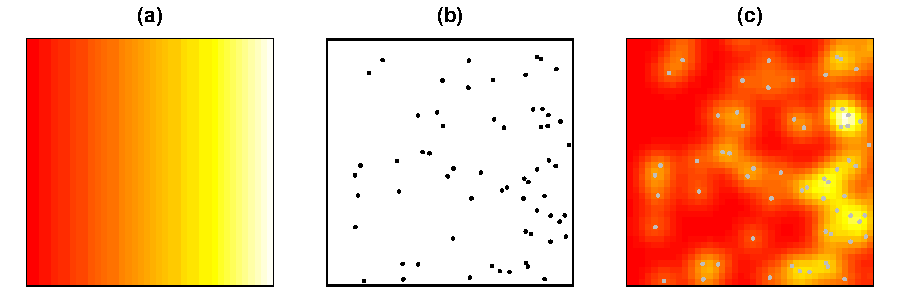
\includegraphics[width=\textwidth]{densities.pdf}
\caption{Examples of (a) an expected activity centre density surface, (b) a realisation of activity centres from this density surface, and (c) the associated realised usage density surface (with activity centres shown as grey dots).}
\label{fig:densities}
\end{figure}

\subsection{Estimated density surfaces}

If we are interested in explaining why density tends to be high in some places and lower in others, or in characterising the process that governs the distribution of activity centres, then we are primarily interested in estimating a density surface like that shown in Figure~\ref{fig:densities}(a). In this example, it is easting that influences this density, but in general it might be any of a wide variety of habitat or environmental covariates, some of which may be unobserved and evidenced only by spatial clustering of activity centres. 

If we are interested only in where the activity centres are, and not in explaining why they are there, then Figure~\ref{fig:densities}(b) suffices. But suppose that we observe activity centres with some error. For example, Figure~\ref{fig:acesterr} shows the distributions of estimated activity centre locations when the locations are estimated with bivariate normal errors with (a) small standard errors, (b) larger standard errors, and (c) standard errors increasing linearly from the centre of the plot. The estimation uncertainty ``spreads'' each activity centre according to a bivariate normal distribution, with greater spreading when there is greater uncerainty.

\begin{figure}[htbp]
\centering
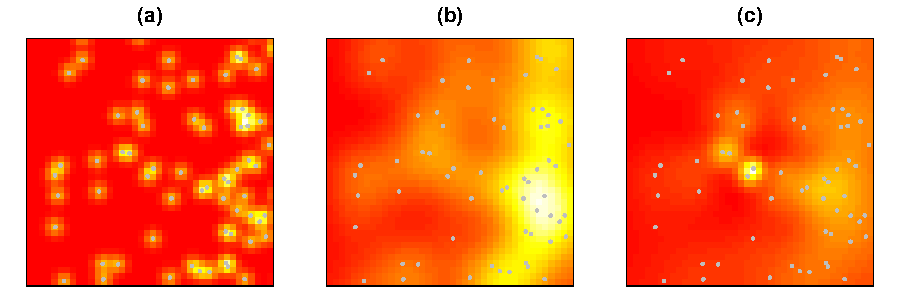
\includegraphics[width=\textwidth]{acesterr.pdf}
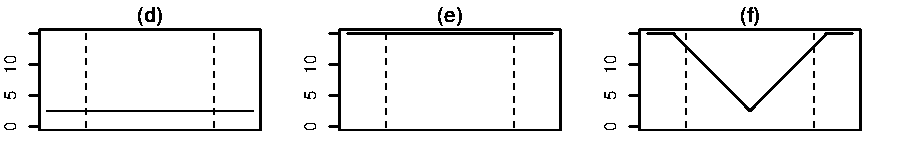
\includegraphics[width=\textwidth]{sigmas.pdf}
\caption{Examples of the density of the activity centres of Figure~\ref{fig:densities}(b), when observed with bivariate normal estimation errors with standard errors (a) $\sigma=2.5$, (b) $\sigma=15$, and (c) $\sigma=2.5$ at the centre of the plot, rising linearly to $\sigma=2.5$ by the edge of the plot. True activity centres shown as grey dots. The colour scales of panels (a) to (c) are such that the highest and lowest densities in each plot is the same.
Panels (d) to (f) plot the standard errors of the observation errors against the x-axis. Vertical dashed lines show the extent of the survey region in panels (a) to (c); a buffer beyond this is included because spreading of points outside it affect the plot within the survey region.}
\label{fig:acesterr}
\end{figure}

Figure~\ref{fig:acesterr}(a) gives a reasonable visual representation of where the activity centres are. It is much more difficult to pick out individual activity centres from Figure~\ref{fig:acesterr}(b), but it gives a reasonable representation of where the high- and low-density regions of activity centres are -- much like Figure~\ref{fig:densities}(a), but customised somewhat for this particular realisation of activity centre locations rather than their long-run average locations. Note, however, that these two figures are representations of exactly the same set of activity centres and that if one interprets them as plots of activity centre density, they contradict each other. Figure~\ref{fig:acesterr}(a) says that almost all the region has low density (red in the plot) and that there are lots of small high-density regions, while Figure~\ref{fig:acesterr}(b) says that there is much less variation in density, that there are large swathes of higher density (the yellow towards the right) and large swathes of low density towards the left. The reason that Figure~\ref{fig:acesterr}(b) shows less variation in density is not that there is less variation in the population (there are exactly the same activity centres in both (a) and (b)), it is that we are less sure about the location of the activity centres in (b). To interpret this as less variation in activity centre density is to invite incorrect ecological inferences.

Now what about Figure~\ref{fig:acesterr}(c)? If this is interpreted as indicating where the high and low-density regions are, it is misleading. It says that the highest density region is in the centre of the plot, and that the region with most variation in density is the central region, which is not true. 

The fact that there is only small observation error in the centre of the plot and large observation error at the edges means that the activity centres near the centre are not spread much and therefore appear as higher peaks in the surface, with low regions where there are no activity centres. Near the edges of the plot, on the other hand, observation error is high and activity centres are spread a lot, which both flattens the peaks at individual activity centre locations and ``fills in'' the troughs where the are no activity centres. We see the same effect with the usage density maps (Figure~\ref{fig:acuseesterr}), but less pronounced because the usage about the activity centres already ``spreads'' around points before any observation error occurs.

\begin{figure}[htbp]
\centering
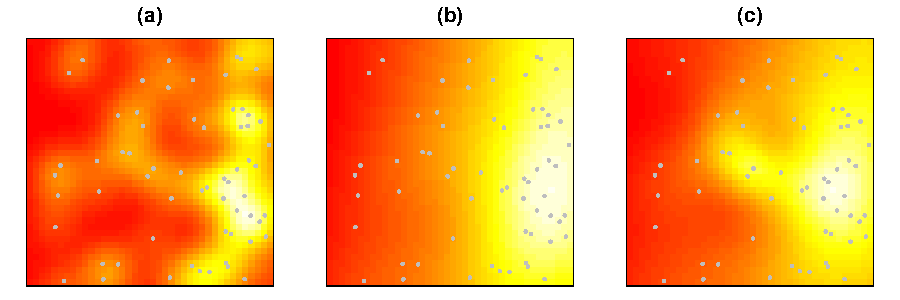
\includegraphics[width=\textwidth]{acuseesterr.pdf}
\caption{Examples of the usage density of Figure~\ref{fig:densities}(c), when observed with bivariate normal estimation errors with standard errors (a) $\sigma=2.5$, (b) $\sigma=15$, and (c) $\sigma=2.5$ at the centre of the plot, rising linearly to $\sigma=2.5$ by the edge of the plot. True activity centres shown as grey dots. The colour scales of the three plots are such that the highest and lowest densities in each plot is the same.}
\label{fig:acuseesterr}
\end{figure}

It is a feature of SCR surveys that the locations of individuals farther from the detector array tend to be estimated with greater uncertainty than individuals within the array. This is illustrated in Figure~\ref{fig:screrr}, which shows the estimated probability density functions for two animals detected on a simulated SCR survey with a 4$\times$4 array placed in the centre of the population shown in Figure~\ref{fig:densities}(b). (The reason contours top right ``avoid'' the triangle is because the detection function range, estimated from the whole survey, not just the points shown, is large and if the activity centre was near the triangle, other detectors would have high probability of detecting it. The fact that they did not makes them ``repel'' the activity centre.) %\todo[inline,size=\footnotesize]{BCS: How come the contours in the top-right are avoiding the black triangle? Shouldn't the contours be happy to cover the triangle, because the animal was detected there?\\ DLB: This is because the detection function range (estimated from the whole survey, not just the points shown) is large and if the activity centre was near the triangle, other detectors would have high probability of detecting it. The fact that they did not makes them ``repel'' the activity centre. I've added this to the text.}

\begin{figure}[htbp]
\centering
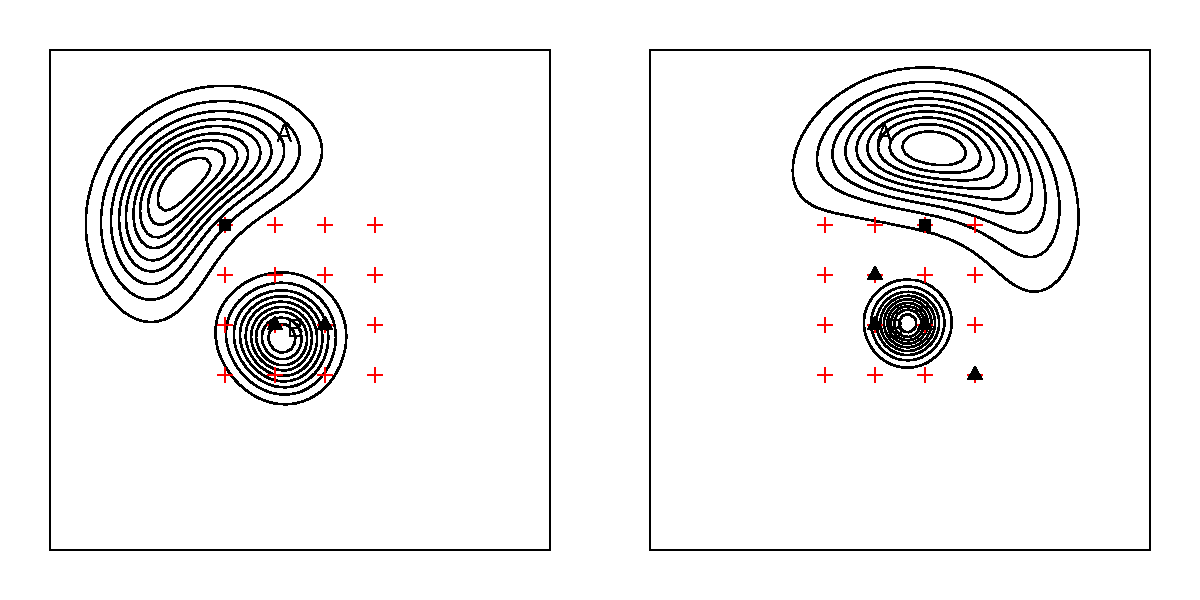
\includegraphics[width=0.5\textwidth]{screrr.pdf}
\caption{Estimated probability density function contours for two detections of an SCR survey of the population shown in Figure~\ref{fig:densities}(b). Traps are shown as red crosses. The lower left individual was detected at traps indicated by black squares, the upper right individual only by the top right trap indicated by a black triangle.}
\label{fig:screrr}
\end{figure}

%FROM BEN: Give examples of papers where people have misinterpreted the sum of posterior AC distributions under either definition (1) or (3) above. Dorazio uses interpretation (1) because they explicitly talk about the distribution of activity centres. Alexander et al. is a little ambiguous, and could be either definition (1) or (3) depending on whether or not they are talking about density under their particular realisation of the state process, but not (2), because they refer to "density of animals" and not "activity centres". Elliot \& Gopalaswamy (2017) do the same thing as Alexander et al. in their caption of Fig 2.

%As a motivating example for the categorisation above, suppose that animals' activity centers have been generated by a point process whose intensity surface is shown in Figure \ref{introplot}a (with intensity increasing eastwards), and with a single realisation of this process overlain (as black dots). In reality the locations of the dots are unknown and must be estimated, but whether the estimated locations of the dots are of interest themselves, or only as a means of estimating the underlying intensity surface, depends on what the goal of the analysis is. If one is interested in where activity centers currently are, one is looking for the dots. If one is interested in which areas are favourable for the location of activity centers {\it in general}, then the dots are only a means with which to estimate the underlying intensity surface. The interpretation of these surfaces differs, but so does their estimation. 

%Expected activity center densities are estimated by modelling the intensity of the state process as a function of environmental covariates, realised activity center densities by summing posterior activity center densities across detected and undetected animals.

%Figure \ref{introplot}b imagines that these realised locations were observed with some small amount of measurement error, and plots the sum of the ``posterior distributions'' for each point that account for this uncertainty. This is -- ignoring for now the complexities of fitting an SCR model -- the surface that we argue is incorrectly interpreted as a species distribution model. It is clearly different to the underlying surface shown in Figure \ref{introplot}a. Figure \ref{introplot}c introduces animal movement around the activity centres, representing the expected density of animals at locations at an arbitrary discrete point in time. The estimation of realised animal densities has not been previously described, but also sums posterior densities across animals (we describe this in more detail in Section ???). The surfaces in Figure \ref{introplot}a-c represent the three kinds of animal density surfaces described above -- expected activity center density, realised activity center density, and realised animal density, respectively. A key point we return to in several places in the paper is that these three surfaces are all of potential ecological interest, but that they differ in fundamental ways, and that it is important to keep the distinctions between the surfaces clear.

%\begin{figure}[htbp]
%\centering
%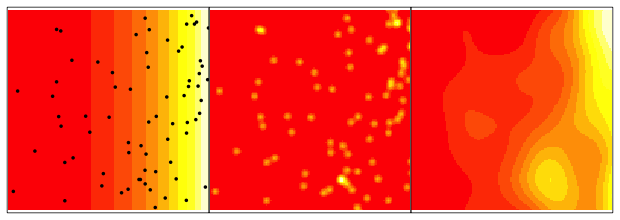
\includegraphics[width=\textwidth]{density-plots.png}
%\caption{Simulated activity centers (black dots, left-hand panel) generated from a point process with intensity increasing from left to right (surface in left-hand panel), estimates of those activity centers (central panel), and estimates of animal locations (right-hand panel). These represent, respectively, what we term expected activity center, realised activity center, and realised animal density surfaces.}
%\label{introplot}
%\end{figure}

%The remainder of the paper illustrates the dependency of the realised activity center density on trap location using three example datasets of increasing complexity. The first (Section \ref{1dbinom}) simulates a fixed number of animals from a one-dimensional binomial point process, assumes that animals do not move and also assumes an extremely simple detection process. This example primarily illustrates that flat density surfaces away from traps reflect a lack of knowledge of the locations of unobserved animals, and not that the realised activity center density is constant.

%The second example (Section \ref{monalisa}) simulates a more realistic two-dimensional Poisson point process. For visual impact our simulated data is drawn from a density surface model based on one of the most recognisable images in Western culture, the Mona Lisa. This example demonstrates that the realised activity center density is dependent on where traps are located, both far from the traps and, perhaps less obviously, in and around the traps. It also introduces the use of covariates as a means of estimating expected activity center densities, and also incorporates animal movement into realised animal density maps.  

%A third and final example (Section \ref{nagarahole}) reanalyses data from a previously published study using SCR to estimate the realised activity center density of tigers in the Nagarahole Tiger Sanctuary \cite{?}. This survey used a dense network of traps; by removing some of these we show the dependency of the density surface on trap locations using real data. A discussion section (Section \ref{discussion}) summarizes our main points, and a final section concludes.



%\section{Simulating a 1-D binomial point process} \label{1dbinom}

%\subsection{Materials and methods}
%We simulate a fixed number of animals distributed across a single dimension according to a linear trend, and then model this data using a binomial point process that incorrectly assumes a uniform distribution of animals across space. Here one can think of, for example, a situation in which true density strongly depends on a covariate that varies in space, but that this covariate is unknown. 

%We place a fixed number of points $N$ at random locations on the interval $0<x<R$, with $R=15$. Points are generated according to a probability density that makes them more likely to appear near $x=0$ than $x=15$ i.e.\ $f(x)\propto 1-x/15$ for $0<x<15$ and $f(x)=0$ otherwise.

%For simplicity we divide the interval into $R=15$ equal-sized regions, thinking of these as cells in a one-dimensional grid. Traps are placed in $T=5$ cells. We make the simplifying assumptions that animals do not move from the cell they are placed in, and that each trap detects animals perfectly within the cell it occupies but cannot detect animals beyond that cell. 

%We simulate with $N=50000$ animals and with different trap configurations.

%\subsection{Results}
%Figure \ref{binom} shows the estimated realised activity center densities -- the estimated number of activity centers for $N=50000$ animals distributed according a binomial point process with density decreasing linearly with $x$. Under the extremely simplified conditions of this example (no movement of animals, perfect detection within cells), SCR recovers the true number of activity centers in each cell that contained a detector, knows how many animals were {\it not} detected\footnote{Here this is because $N$ is known but if $N$ is unknown it can be estimated. A model assuming a constant density and detecting $n$ animals from a perfect survey of $T/R$ of the study area estimates the total number of animals to be $\hat{N}=n/(T/R)$, implying there are $\hat{N}-n$ animals in the area that were not detected by any trap.}, and distributes the activity centers of these undetected animals evenly across the cells that do not contain a detector\footnote{$\hat{N}-n$ activity centers distributed uniformly between $R-T$ trapless cells gives a mean of $(N-n)/(R-T)$ activity centers per cell, close to the mean of the underlying process $N/R$ when $n\ll N$ and $T\ll R$, as would usually be for wildlife surveys.}. 

%\begin{figure}[htbp]
%\centering
%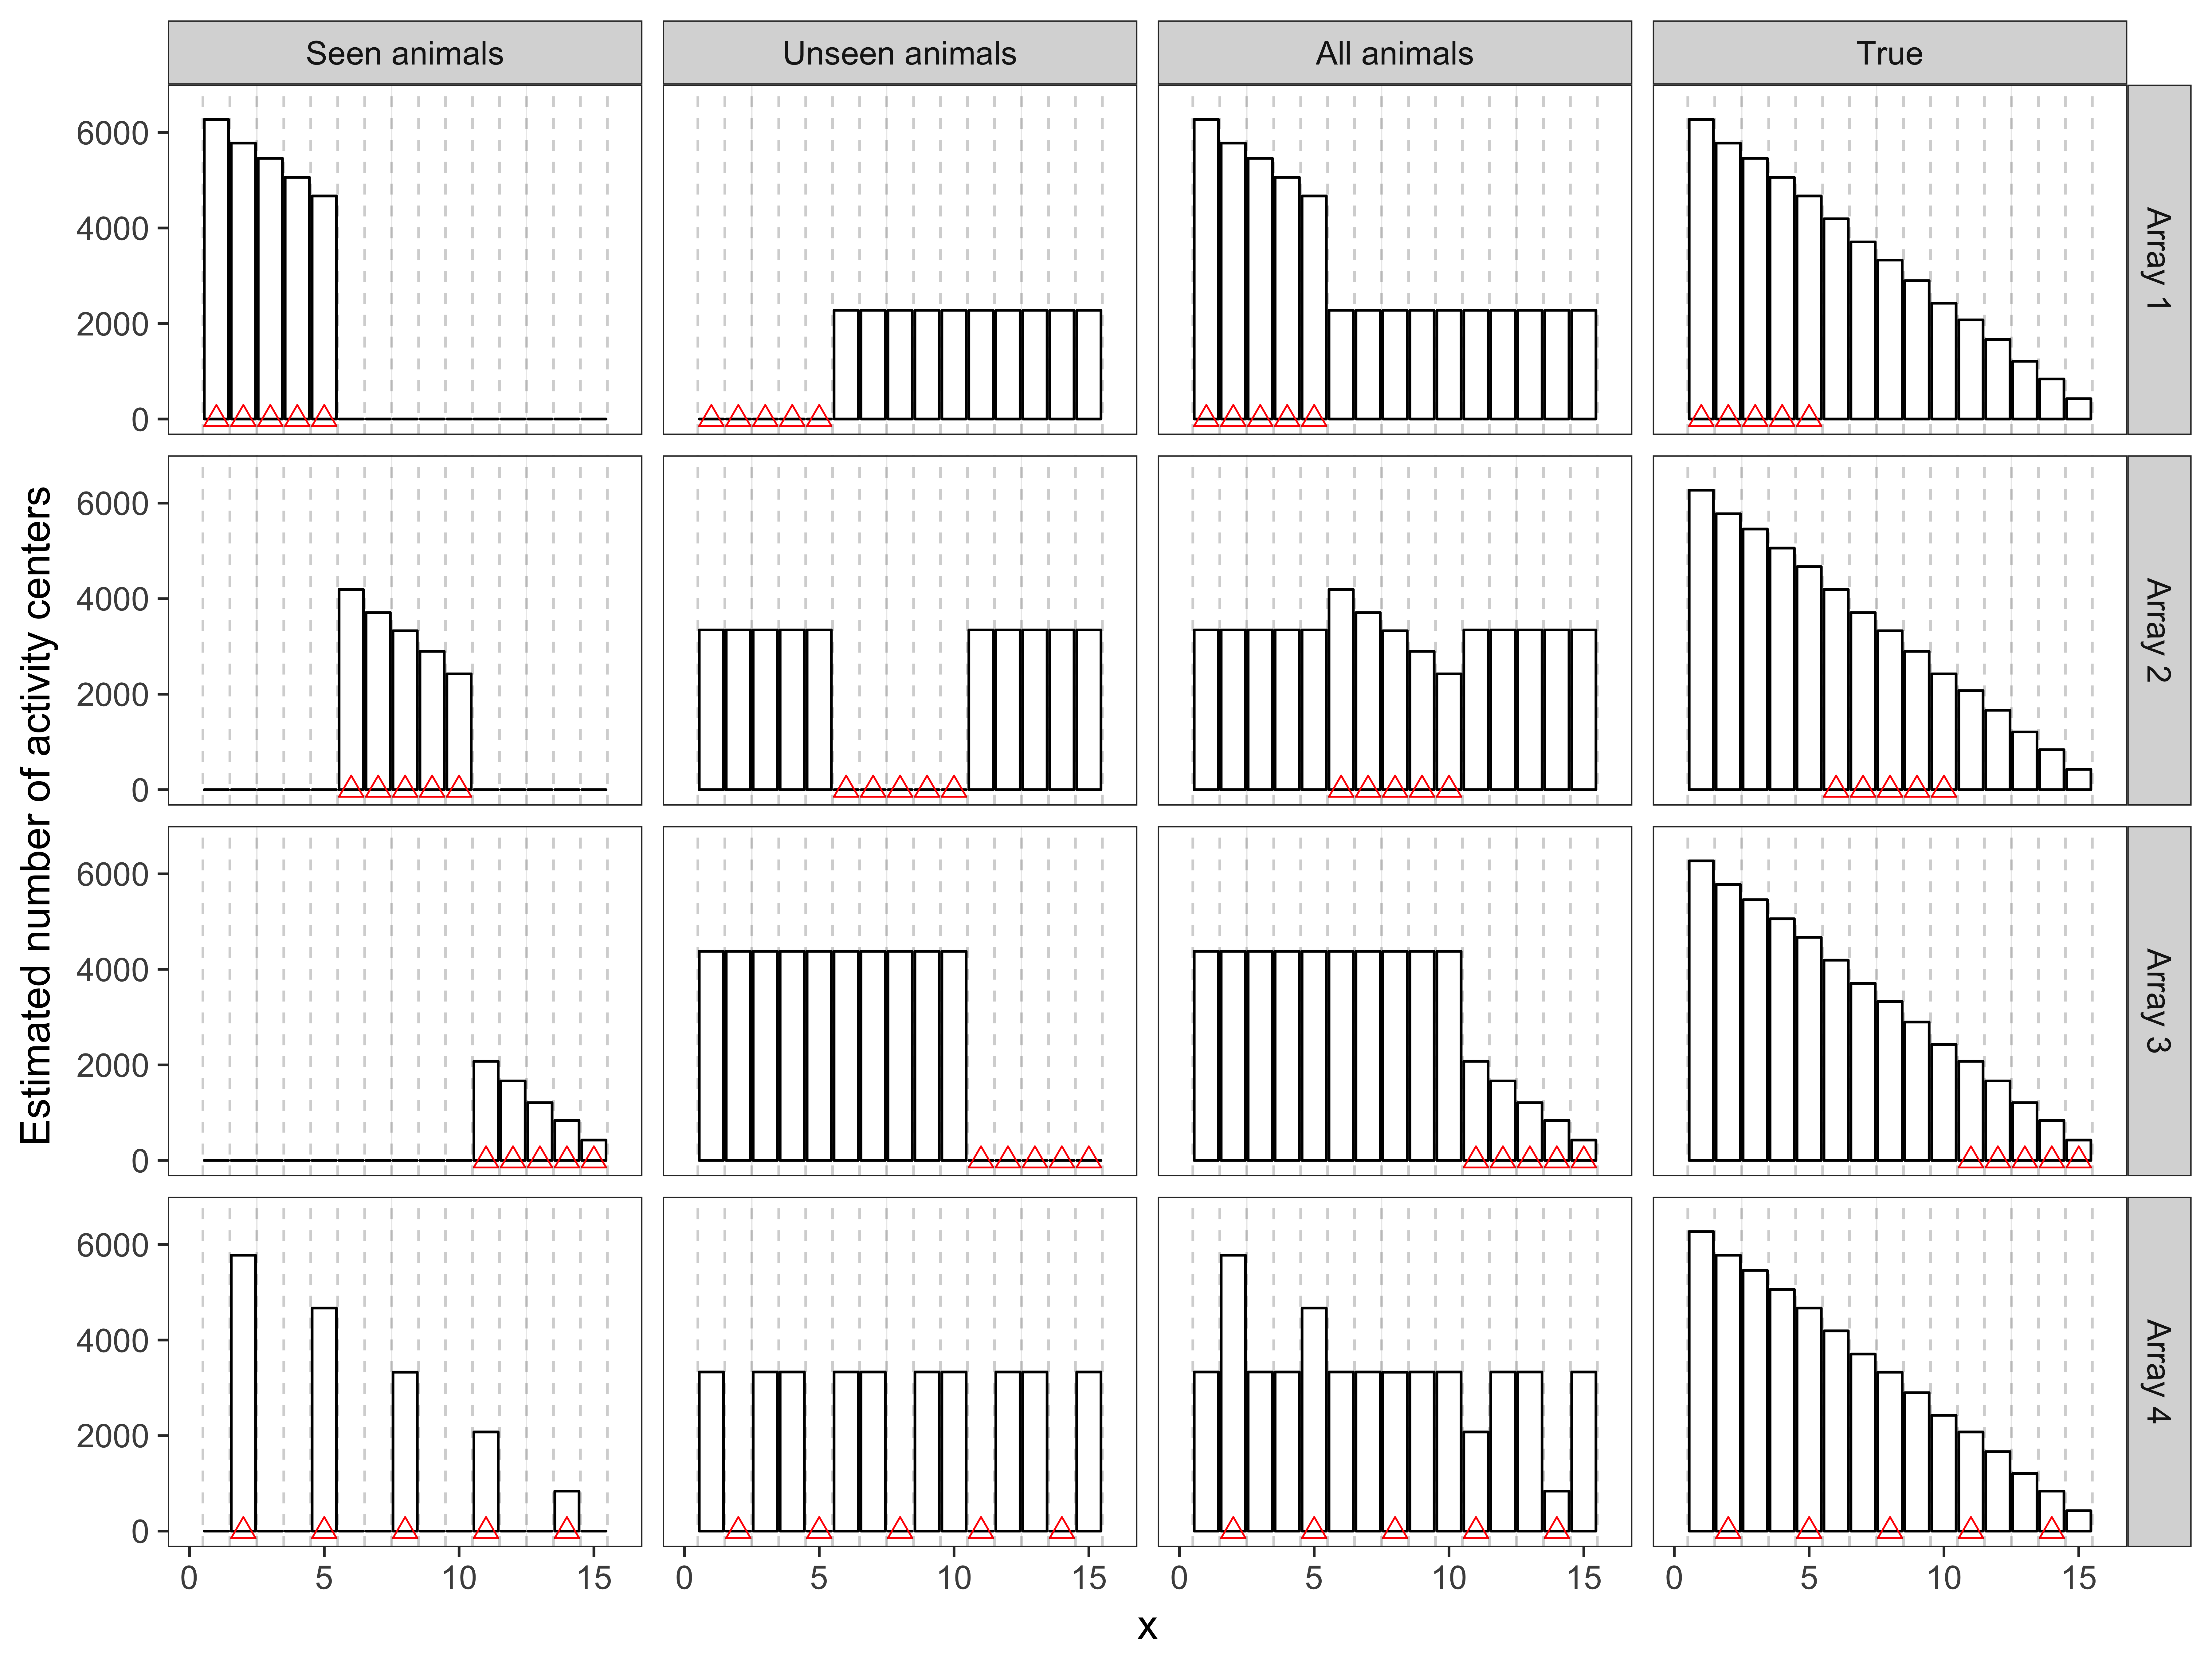
\includegraphics[width=1\textwidth]{binompp_inf.png}
%\caption{Estimated numbers of activity centers obtained from a binomial point process with $N=50000$ simulated animals and density decreasing linearly with $x$, no animal movement, and a step detection function that is perfect within cells and zero otherwise.}
%\label{binom}
%\end{figure}

\section{SCR density estimation methods}

Maximum likelihood (ML) and Bayesian SCR estimation methods are documented in a good number of papers, starting with \cite{Borchers+Efford:08} and \cite{Royle+Young:08}, and we do not repeat the details here. Both ML and Bayesian inference are based on SCR likelihood functions that include a component specifying the activity centre density surface, which may depend on spatially-referenced covariates. (The linear density surface shown in Figure~\ref{fig:densities}(a) is an example.) The density surface is typically of the form $D(\bm{s})=\exp\left\{\beta_0 + \sum_{k=1}^K\beta_kx_k(\bm{s})\right\}$, where $\bm{s}$ is a point in the plane, $x_k(\bm{s})$ is the $k$th of $K$ spatially-referenced covariates, evaluated at $\bm{s}$, $\beta_0$ is and intercept parameter, and $\beta_k$ is the slope parameter for the $k$th spatially-referenced covariate. ML and Bayesian methods are able to estimate $\beta_0,\ldots,\beta_K$, and hence to estimate the density surface. We refer to this as the ``estimated density surface''.

Given spatial capture histories, ML and Bayesian methods are also able to estimate the locations of activity centres. (Locations like those shown in Figure~\ref{fig:densities}(b), for example.) While activity centres are points, there is always uncertainty associated with estimating their locations, so that SCR estimates of activity centre locations are probability density functions (PDFs), not points. Estimates of these PDFs are conditional on the spatial capture histories of the individuals concerned -- because the capture histories contain information on where each animal's activity centre was (see the capture histories and estimated location densities in Figure~\ref{fig:screrr}, for example). Details of how one obtains these estimated activity centre PDFs are contained in Section 4.3 of \cite{Borchers+Efford:08} for ML methods and the section ``Estimating derived parameters'' on page 3238 of \cite{Royle+al:09b} for Bayesian methods.

Note that we can obtain activity centre PDFs for undetected animals, because although the animals were unobserved, we know their capture histories -- namely no capture at every detector. Note also that all undetected animals will have the same activity centre PDF\footnote{This is not the case if there are individual-level covariates that affect detection probability estimates, but this is a complication that we ignore here in order to present as clear and uncomplicated an exposition of they key points of this paper as we can.} because they all have the same capture history. 

Suppose that we estimate from an SCR survey that there are $\hat{N}$ animals within the survey region. If one adds up the activity centre PDFs for all $n$ detected animals, and the $\hat{N}-n$ activity centre PDFs of the undetected animals, at all points in the survey region, one gets a surface that is in many publications (including those lised in the Introduction) interpreted as a density surface for animal locations.  We refer to this as the ``estimated activity centre \textit{location} surface''.

What we call an ``estimated activity centre \textit{location} surface'' has been referred to as the estimated distribution, or density of \textit{animals}. However, animals distribute themselves around their activity centres, so that activity centre density and animal density are not the same thing. Suppose for example, that we are certain that there is exactly one activity centre in a region that has surface area 1 (so that activity centre density in this region is 1). Suppose also that the animal with activity centre in this region ranges wider than this region, and spends exactly half its time in this region. It is not certain that there is an animal in the region at any time, so that animal density will be less than 1. In this example, it would be fair to say that the \textit{animal} density in the region is 0.5. To avoid confusion, we refer to this as the ``usage density'' rather than ``animal density''. Details of how one obtains an estimated usage denstiy surface from an estimated activity centre \textit{location} surface are given in Appendix~\ref{appx:usage-details}.\todo[inline,size=\footnotesize]{Ben/Ian: Can you insert mathematical details? I think we need to do this because there are (to my knowledge) no publications that contain the details. BCS: Sure thing, I'll fill it in here. Basically it's just spreading the point around in the same way you have above for estimation uncertainty. I'm pretty sure this is linked to the idea of what some people call a `utilisation distribution'; I'd better do a little reading about these, too.}

In summary, there are three kinds of estimated surface of interest here: 
\begin{itemize}
\item The \textbf{estimated activity centre \textit{density} surface}: This is an estimate of the density model component of the SCR model, which governs the location of activity centres.
\item The \textbf{estimated activity centre \textit{location} surface}: This is the combined estimated activity centre densities of all animals, conditional on each animal's capture history.
\item The \textbf{estimated usage surface}:  This is the combined space usage density of animals, conditional on each animal's capture history.
\end{itemize}



\section{Methods}

We illustrate what each of the three kinds of estimated surface gives the practitioner, and what interpretations of the surfaces are valid and useful, by (a) simulating data from a density surface that has easy visual interpretation, and (b) using the Ngarahole SCR tiger survey data kindly provided by the first author of \cite{Dorazio+Karanth:17}.

\subsection{Reproducing the Mona Lisa} \label{monalisa}

For easy visual interpretation, we turned one of the most recognisable images in Western culture, the Mona Lisa, into a density surface. We created a greyscale version of a region of the original image (Figure \ref{mlinputs}, ``True Density'') in which greyscale values give the true density of activity centres, and lighter areas correspond to higher densities.

We then used the density surface to generate two realisations of points from the underlying process. In the first of these we generated the number of points from a single draw from a Poisson distribution with mean 7,500, resulting in 7,451 activity centres being generated, which we plot in Figure \ref{mlinputs}, ``Realisation 1'' as a density at $50\times 50$ pixel resolution. This realisation has the advantage of closely reproducing the source image, and when we conduct SCR surveys with this population, it gives us an indication of the asymptotic behaviour of SCR density estimators, i.e. as sample size gets very large. We also generated a much smaller second realisation of 84 points (Figure \ref{mlinputs}, ``Realisation 2''). This realisation captures the Mona Lisa only at an extremely gross level (the darkest region corresponding to the hair can be picked out if you squint at the image long enough!), but is a useful aid to understanding some properties of the estimators.

\begin{figure}[htbp]
\centering
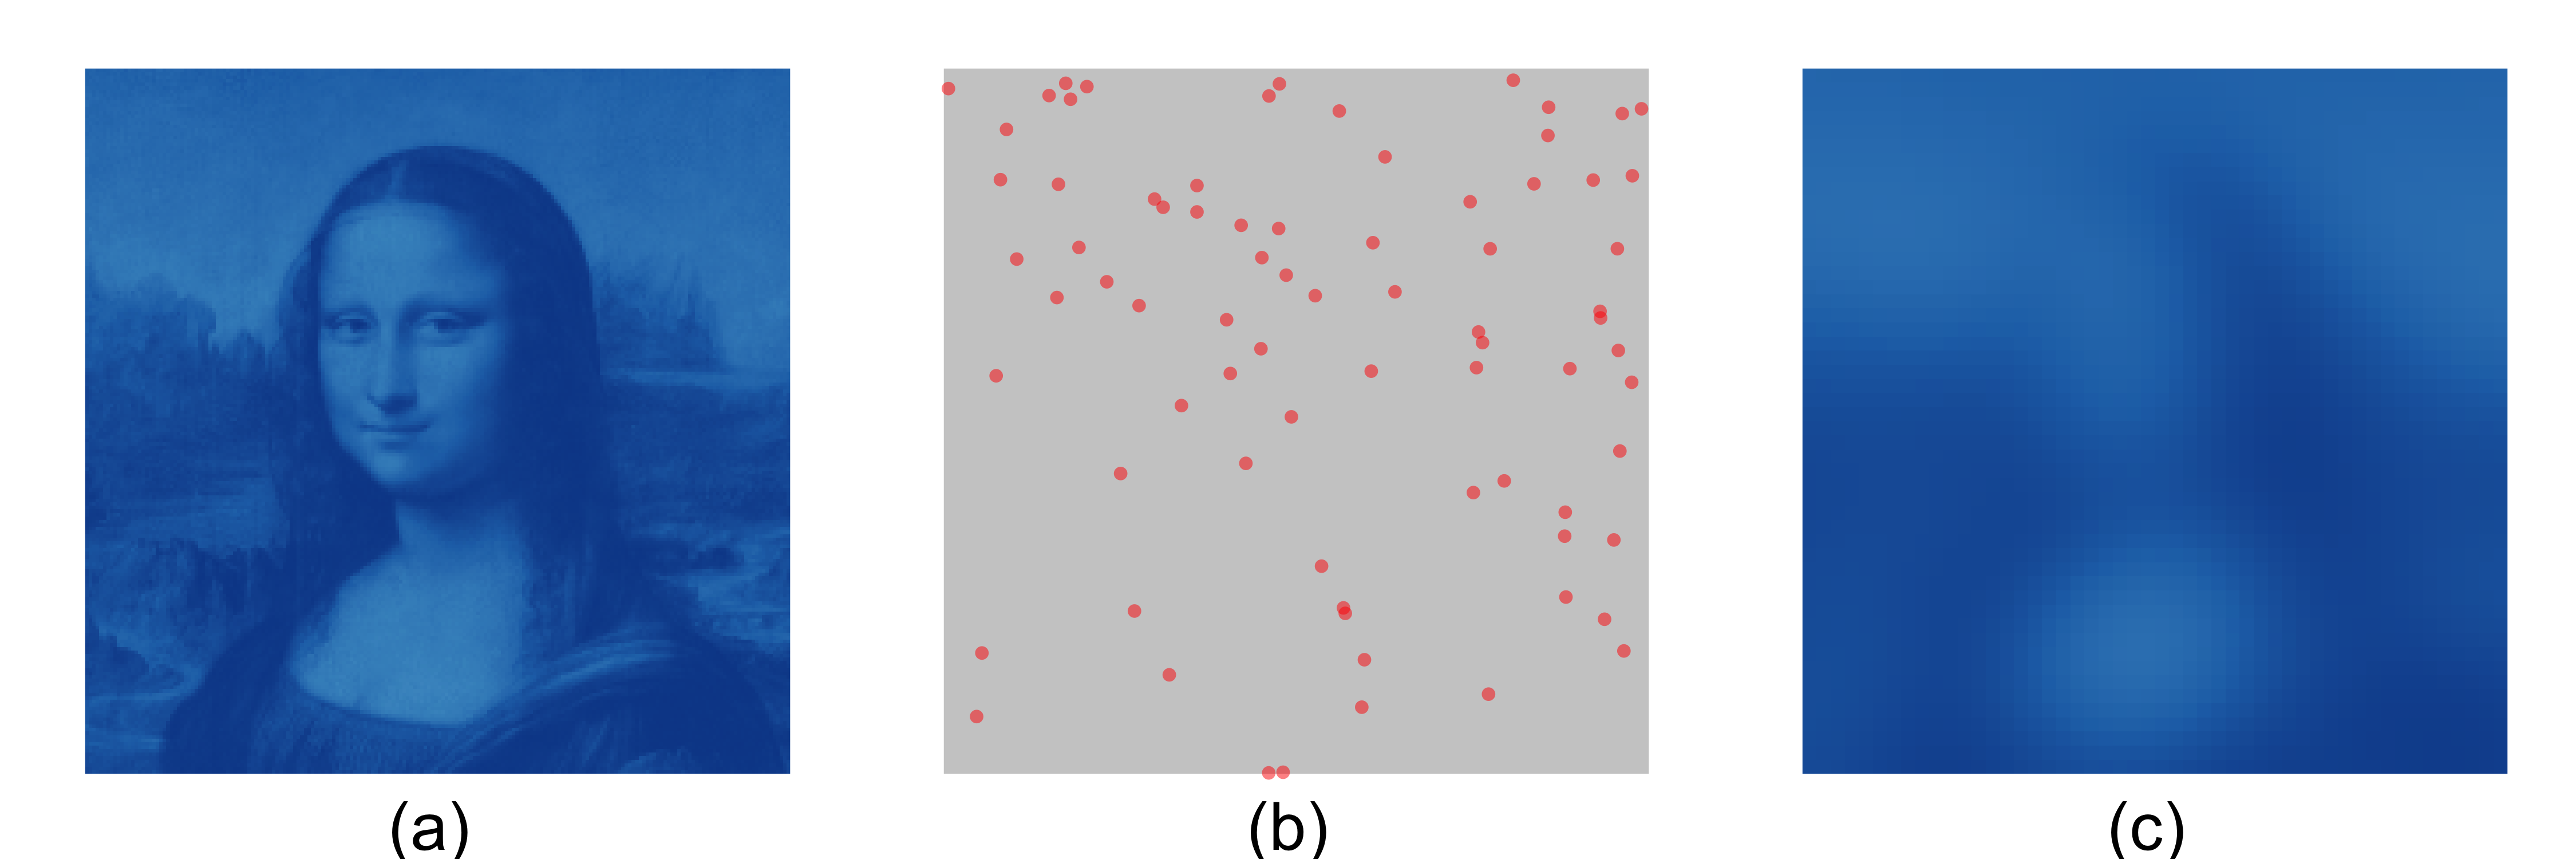
\includegraphics[width=1\textwidth]{mona_inputdata.png}
\caption{Input data for the Mona Lisa simulation study. A grayscale version of the Mona Lisa (``True Density'') is treated as an activity centre density surface, frwom which we generated a sample of 7,451 and 84 activity centres and plotted these as densities at $50\times 50$ pixel resolution (``Realisation 1'' and ``Realisation 2'', respectively).}
\label{mlinputs}
\end{figure}

We simulated SCR surveys of the population, using a variety of detector arrays and also varying the number of detection occasions.\todo[inline,size=\footnotesize]{I think occasions are a red herring here. If these are count data, then occasion is irrelevant. What we should report is the sample size (total number of detections and number of unique individuals detected).} Different arrays and detection functions \todo{DLB: Or encounter functions?} were used for the large and small populations described above. With the large number of activity centers, we used four different 3x4 arrays (Figure \ref{mona1low}), with array centers $(19,21)$, $(19,33)$, $(28, 21)$, or $(28, 33)$. All arrays were spaced such that they have length 8 in the $x$-plane and 12 in the $y$-plane, and so have an average spacing of $4=2\sigma$. We simulated capture histories using a half-normal detection function with $g_0$, the probability of detection at a single detector placed at an activity centre, set to 0.5, and $\sigma$, the spatial scale parameter, set to 2. We then simulated a capture history for either one or 20 occasions on each array.\todo[size=\footnotesize]{Same comment about occasions applies - and 20 occasions is very rare, so not great example in this way.}\todo[inline,size=\footnotesize]{BCS: I had a look at some R code, and I think I saw that the hazard halfnormal detection function was being used by defining $\lambda_0$ and $\sigma$. Or maybe this was just a default setting? Anyway I'm just leaving this comment here to remind me to have a look at the code later (or Ian can clarify).}

When using relatively few activity centers, visual interpretation was made easier by increasing the spatial scale parameter, effectively increasing the distance animals travel from the activity centers, and also by increasing the distance between detectors. For these cases, we increased $\sigma$ to 4, holding other detection function parameters at their previous values, and used a 3x4 array centered on $(18,34)$ and with an average spacing of 8 between detectors, double that used previously. We simulated capture histories after one, three, ten, and 20 occasions\todo{Same comment about occaions applies.}. 

After simulating these capture histories for these arrays, we  created an estimated activity centre surface for each simulation. In this scenario we assumed a model with constant density and compared the resulting estimated realised activity center surface to the true population density surface (the Mona Lisa).

The next step was to introduce covariates into our density model. We generated covariates by manipulating the ``Low Res'' image to obtain further images using simple image processing operations like blurring and shifting\todo{DLB: I thoink we should remove the shifting}. Covariates are thus all functions of the true densities but the strength of the association between the covariate and true density varies substantially. We generated four covariates: a ``strong'' covariate that uses a Deriche (blur) filter with a small range, effectively smoothing the image locally; a ``moderate'' covariate that uses the same blur filter but with a larger range, increasing the amount of smoothing; a ``weak'' covariate that uses the same degree of blurring as the moderate covariate but in addition shifts the image down and to the right, destroying much of the relationship between covariate and density; and a ``locally strong'' covariate, which uses the strong covariate values in the top right hand part of the image and the weak covariate values in the remainder of the image. These covariates are shown in the first row of plots in Figure \ref{covariates}. For each covariate we estimated a corresponding expected activity center density.

We simulated capture histories and created an estimated realised animal density surface i.e.\ including movement, for each of these simulations and compared them to the true population density surface. All computations were done using the {\it secr} package in R version 3.4.3. 

\subsection{Results}

\subsubsection{Estimated realised activity centre densities with many activity centers}

The same patterns hold in two dimensions under the standard wildlife survey assumptions of Poisson-distributed activity centers (with constant intensity) and detectability inversely related to distance from activity center (Figure \ref{mona1low} and \ref{mona1hi}). A single sampling occasion was sufficient to capture the broad features of the Mona Lisa, but only close to where detectors were located (Figure \ref{mona1low}, first row). Away from the detectors the estimated density quickly reverted to close to the estimated mean intensity of the process. Additional sampling occasions resulted in the density of activity centers close to detectors being estimated in much greater detail, but did not affect the surface away from detectors (Figure \ref{mona1hi}, first row). 

Very different relative and absolute densities were obtained depending on where traps are located, even when estimating density {\it in exactly the same region of the surface and where that region is close to the array} (Figure \ref{mona1low} and \ref{mona1hi}, second row). With a single occasion, density was always estimated to be highest nearest the corner where the trap is located (Figure \ref{mona1low}, second row). This pattern occured because the inset region happened to occur in a region of above average density. If instead it occured in a low density region one would see the opposite pattern -- low density in the corner containing a trap, increasing away from the trap. This was clearly visible when a single sampling occasion was used, because the estimated surface reverted quickly to the mean intensity. Additional sampling allowed fine detail in the density surface to be estimated close to traps, with slower reversion to mean intensity, but there was still very clear disagreement between the density surfaces returned by the different arrays (Figure \ref{mona1hi}, second row).

\begin{figure}[htbp]
\centering
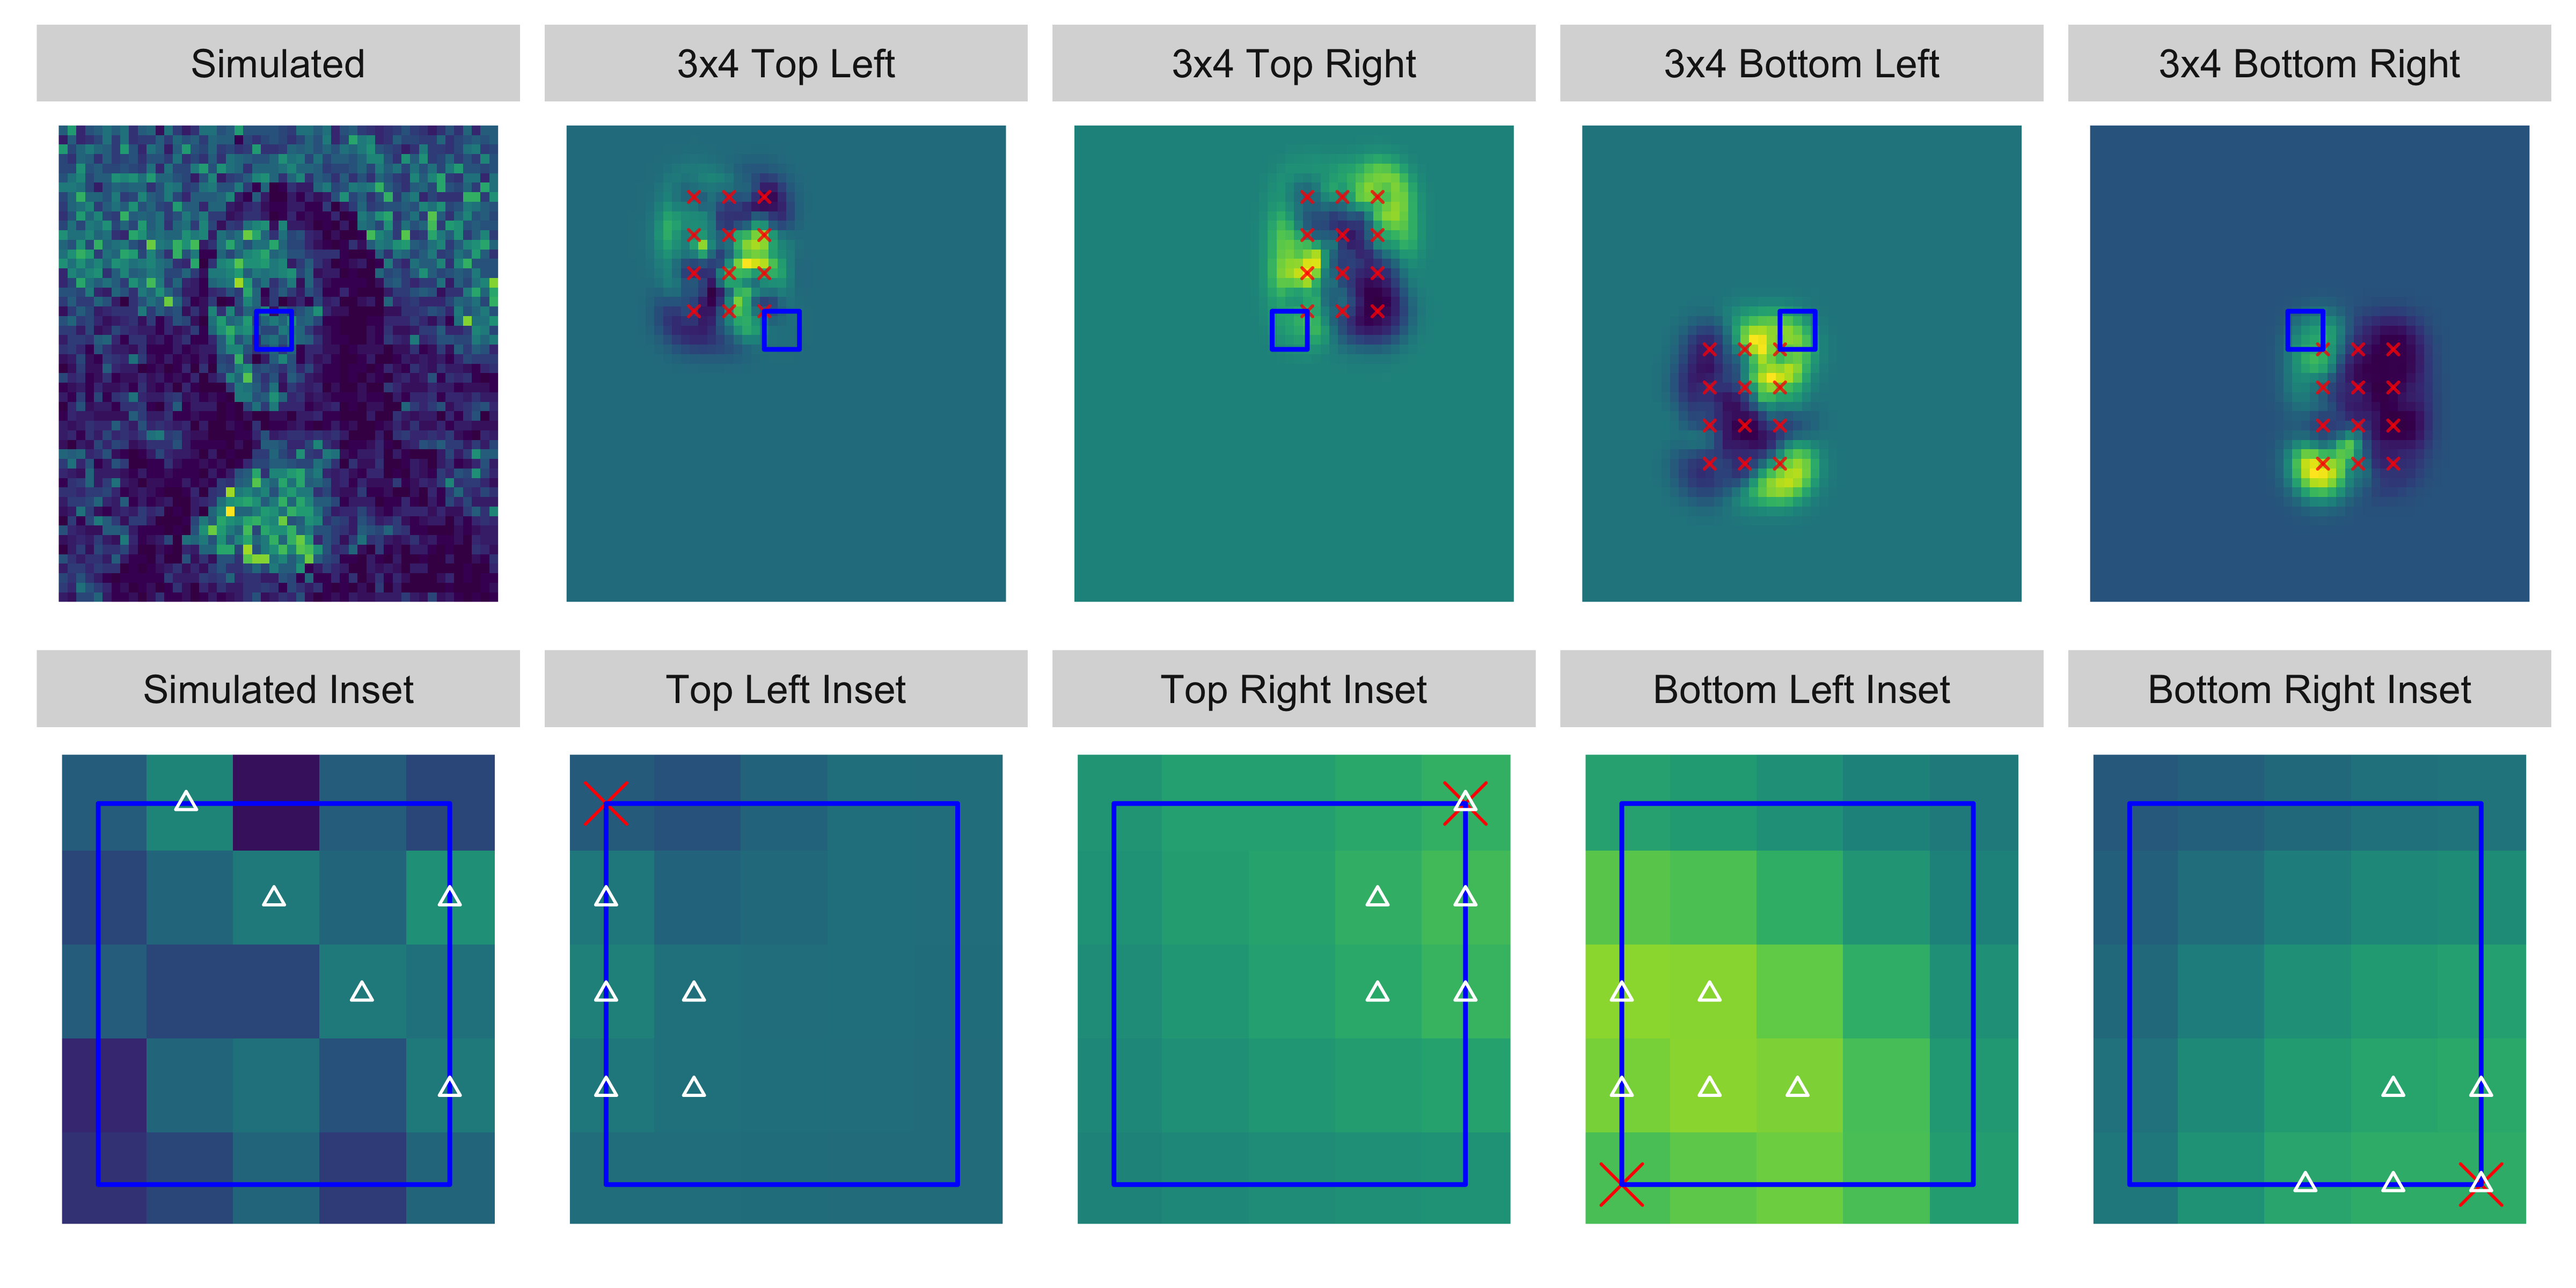
\includegraphics[width=1\textwidth]{many_faces_mona_loweffort.png}
\caption{True activity center densities in this realisation (``Simulated'') compared with realised activity center surfaces estimated using different arrays after a single sampling occasion. High density areas are indicated in yellow, low density areas in blue. Detectors are shown as red crosses. Blue squares show the same 4x4 square centered at $(25,29)$, whose vertices are corner detectors from each of 3x4 arrays. Each plot in the second row shows an enlargement of the blue square in the plot above it. White triangles denote the five cells with the highest estimated densities in each of the second row plots.}
\label{mona1low}
\end{figure}

\todo[inline,size=\footnotesize]{The densities in these plots should really be expected densities (i.e. averages over lots of simulations) - particularly for the bottom row of estimates, since you might expect substantial random variation in these from sample to sample. The top images illustrate fairly convincingly how the SCR ``torch'' does pretty well where it ``shines'' but can't see beyond, without the need to use expected values, but because you can't see pattern in the bottom ones, you are more inclined to say ``So what that they are not the same - there is sampling variation.''
Also, we need to give sample sizes for these surveys (number detections and number of different individuals).}

\begin{figure}[htbp]
\centering
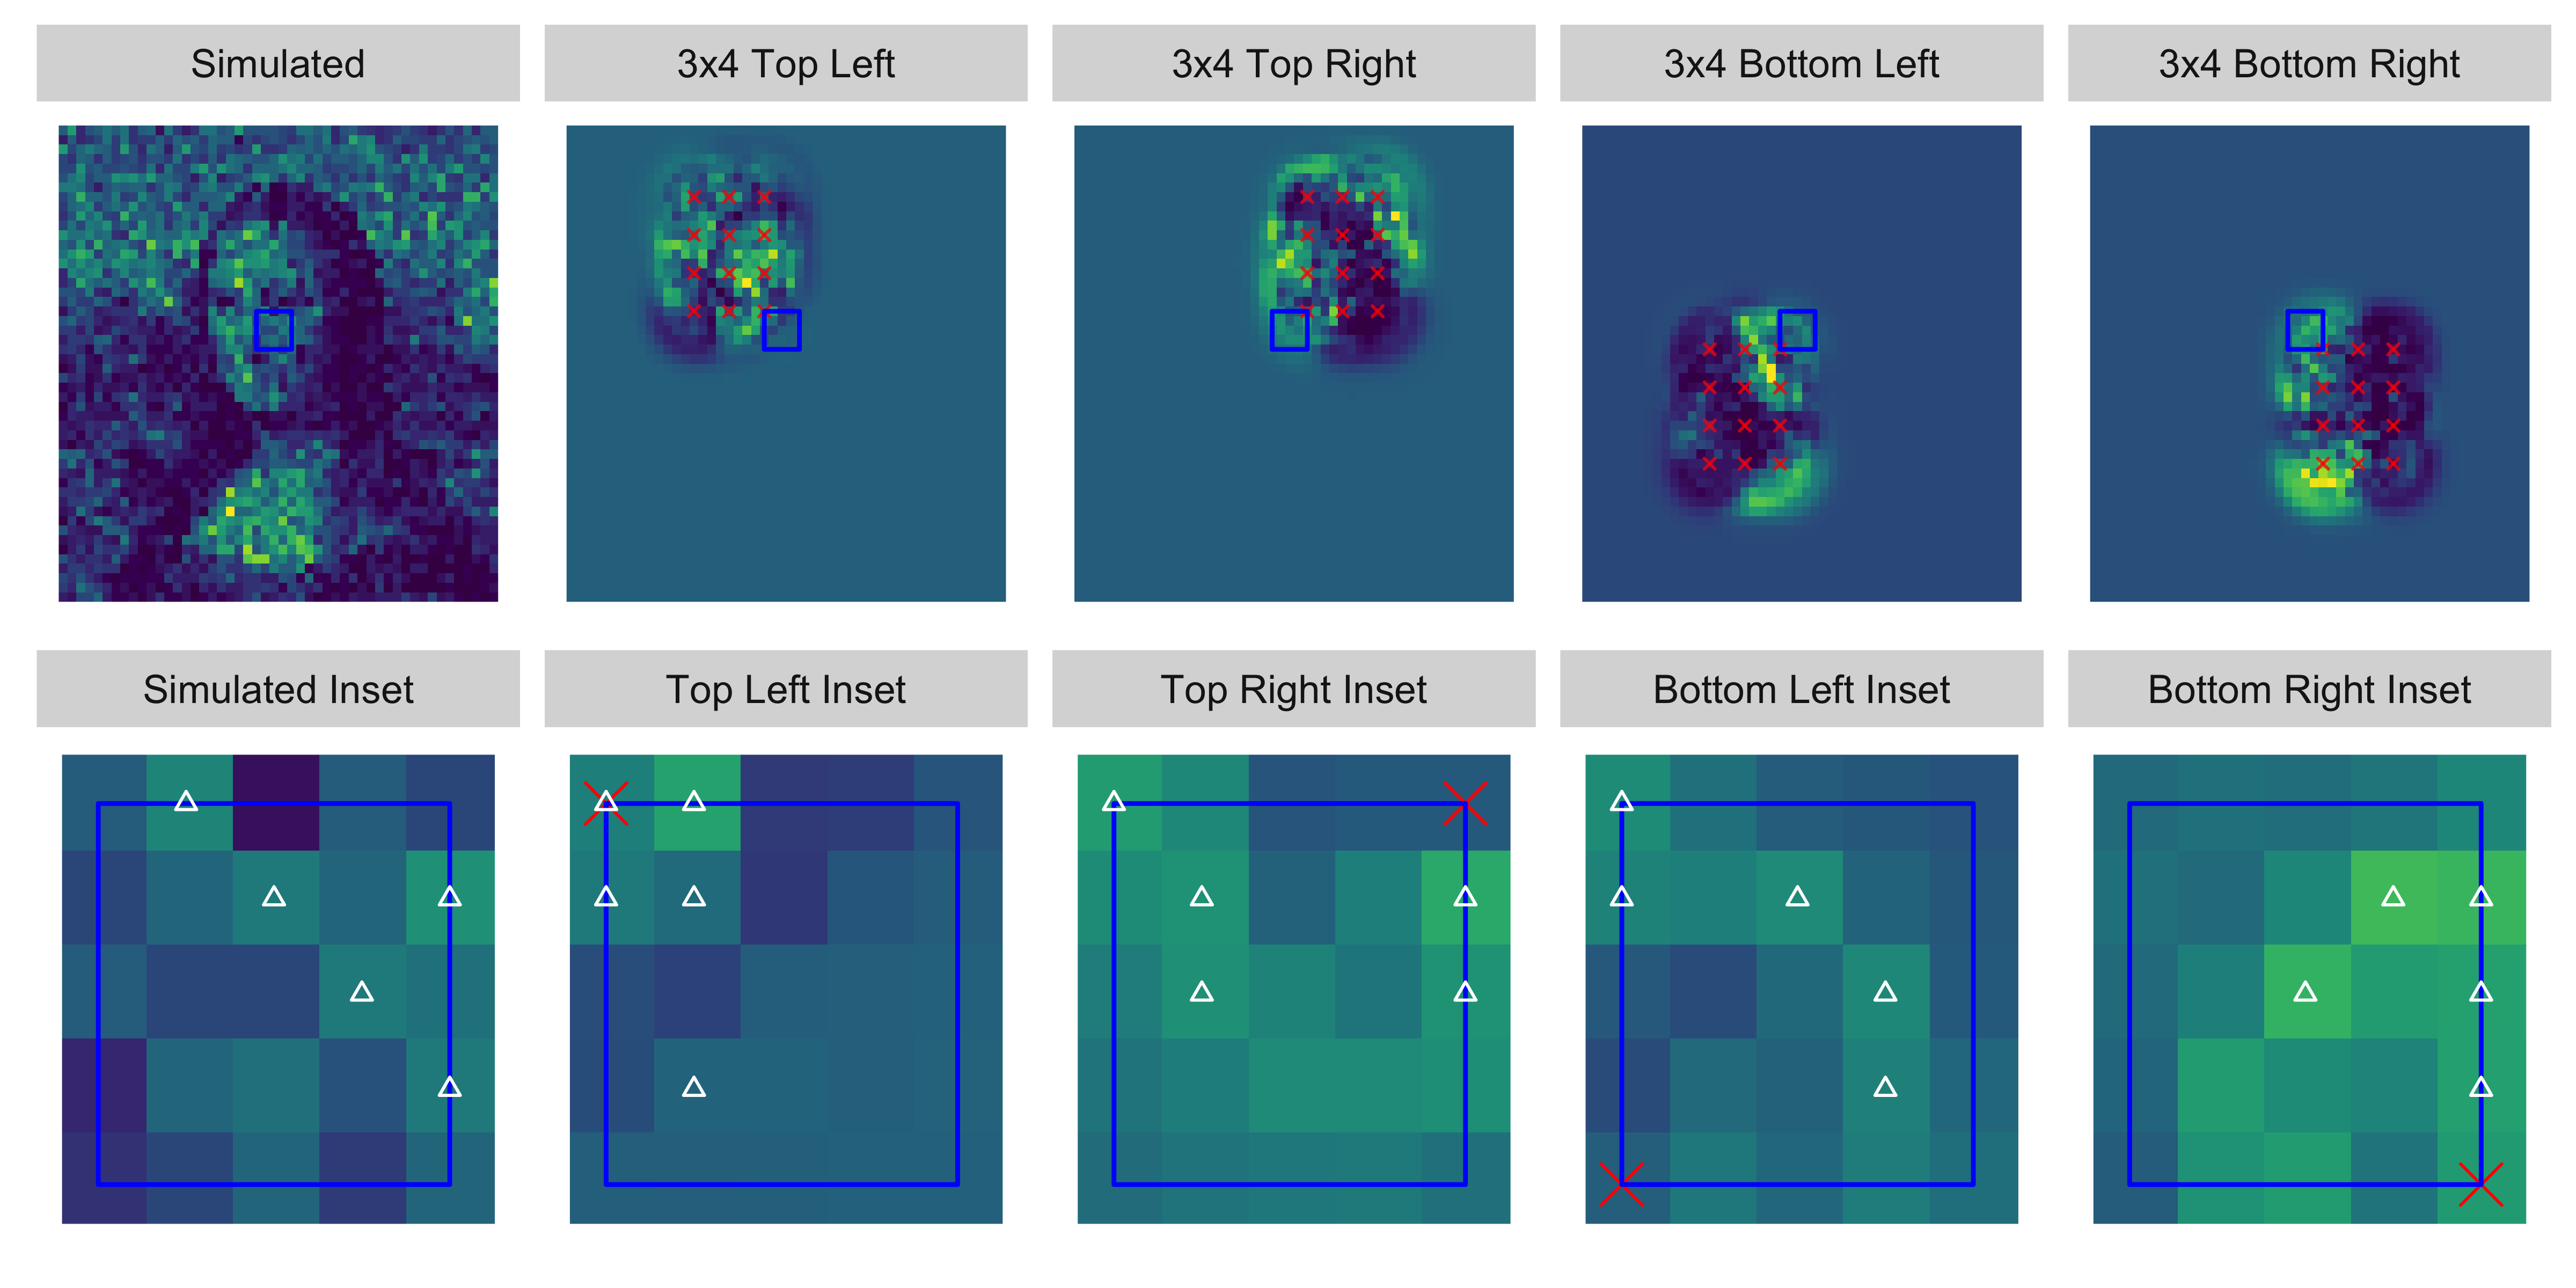
\includegraphics[width=1\textwidth]{many_faces_mona_higheffort.png}
\caption{True activity center densities in this realisation (``Simulated'') compared with activity center surfaces estimated using different arrays after 20 sampling occasions. High density areas are indicated in yellow, low density areas in blue. See the caption to Figure \ref{mona1low} for further annotation details.}
\label{mona1hi}
\end{figure}

\subsubsection{Estimated expected activity center densities with many activity centers}

Introducing covariates into the density models allowed us to recover features of the Mona Lisa across the entire image, not just near where detectors were located, although good estimation of activity center locations depended heavily on the availability of good covariates (Figure \ref{covariates}). With our ``strong'' covariate we recovered all of the broad features of the Mona Lisa, and many of the fine scale features such as eyes, shading of clouds, {\it etc}. With the ``moderate'' covariate we recovered broad scale features but no finer details. With a ``weak'' covariate, the estimated density surface essentially reverted to the mean intensity of the process across the entire region. With a ``locally strong'' covariate -- one that is a good indicator of density in some parts of the study region but poor elsewhere -- the dependency on array location was reintroduced. If the array was located where the covariate was strong, the estimated density surface was accurate in that vicinity. If the array was located where the covariate was weak, then the model estimated no relationship between covariate and density and reverted back to the mean intensity everywhere in the region (Figure \ref{covariates}). 

\begin{figure}[htbp]
\centering
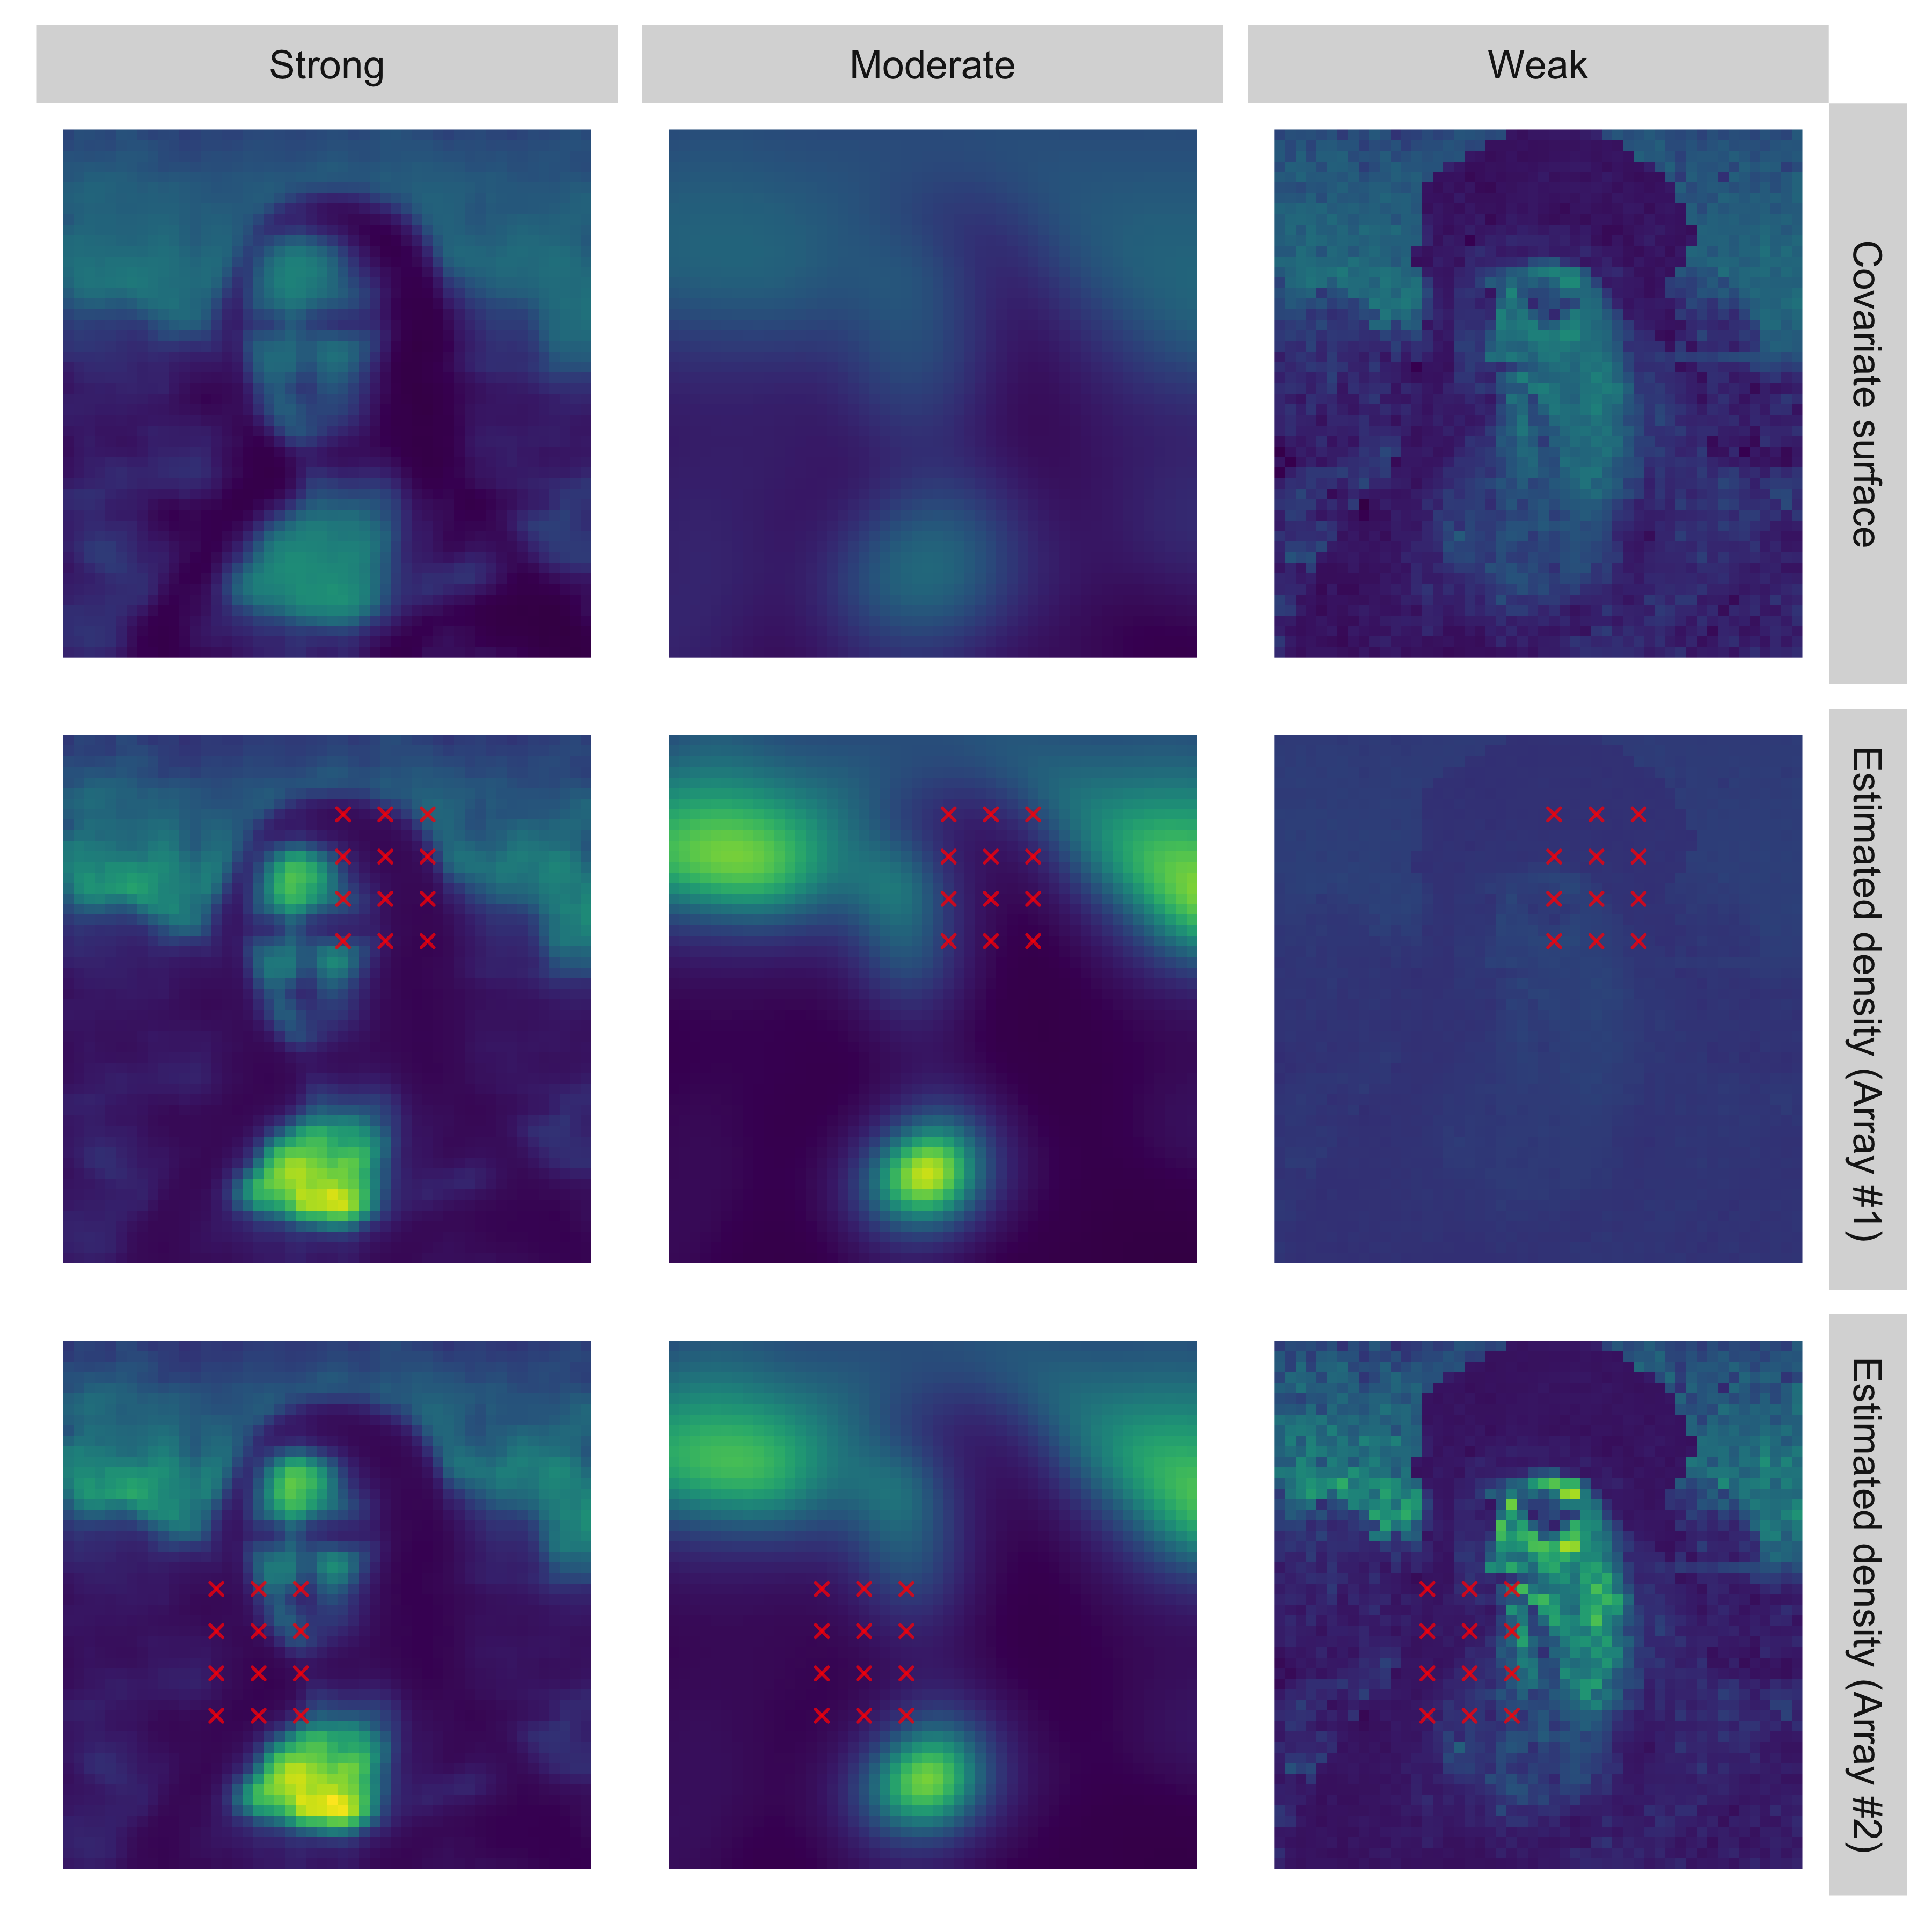
\includegraphics[width=1\textwidth]{mona_covariates.png}
\caption{Expected activity center surfaces estimated using a model with density a function on one of four simulated spatially-varying covariates. Covariates are shown in the first row of plots, and were generating by manipulating the true intensity surface (Figure \ref{inputdata}, ``Low Res'') by blurring and shifting operations (see Section \ref{s:simcapthist} for details). High density areas are indicated in yellow, low density areas in blue. Detectors are shown as red crosses.} 
\label{covariates}
\end{figure}

\subsubsection{Estimated realised activity centre densities with few activity centers}

We observed similar patterns under the more ``wildlife survey appropriate'' condition in which we generated only 85 activity centers across the study region (Figure \ref{peaky}). In this case there is a large difference between the mean intensity surface (the Mona Lisa) and the activity center surface in this realization (85 points), and so it is not surprising that the estimated realised activity centre density surface looks nothing like the Mona Lisa (Figure \ref{peaky}, first row). Nevertheless, a model assuming constant density gives increasingly accurate estimates of the locations of activity centers in the vicinity of detectors as survey effort increases, but very little information is obtained elsewhere, and this does not change with survey effort (Figure \ref{peaky}, first row). This gives the estimated activity center surfaces a characteristic pattern -- the surface becomes increasingly peaked or ``spiky'' around detectors as survey effort increases, but remains flat away from the array. 

\subsubsection{Estimated expected animal densities with few activity centers}

Any covariate model returns a surface that is some multiple of the covariate surface. Whether this is a good approximation of the true mean intensity surface depends on the strength of the covariate and sample size. With a strong covariate and sufficient sampling occasions we recovered the Mona Lisa, but with only a single occasion the direction of the relationship was incorrectly estimated, so that dark areas were predicted as light and light areas as dark (Figure \ref{peaky}, second row). This error was corrected by additional occasions. The same pattern occured with a moderate covariate, but the effect of the weaker covariate is clear in that we did not recover as good an approximation of the Mona Lisa (Figure \ref{peaky}, third row). Additional sampling would not help with this. Note that in both cases the surface we recovered is an approximation of the mean intensity surface. It does not give a good approximation to the locations of the 85 activity centers in this particular realization.

\begin{figure}[htbp]
\centering
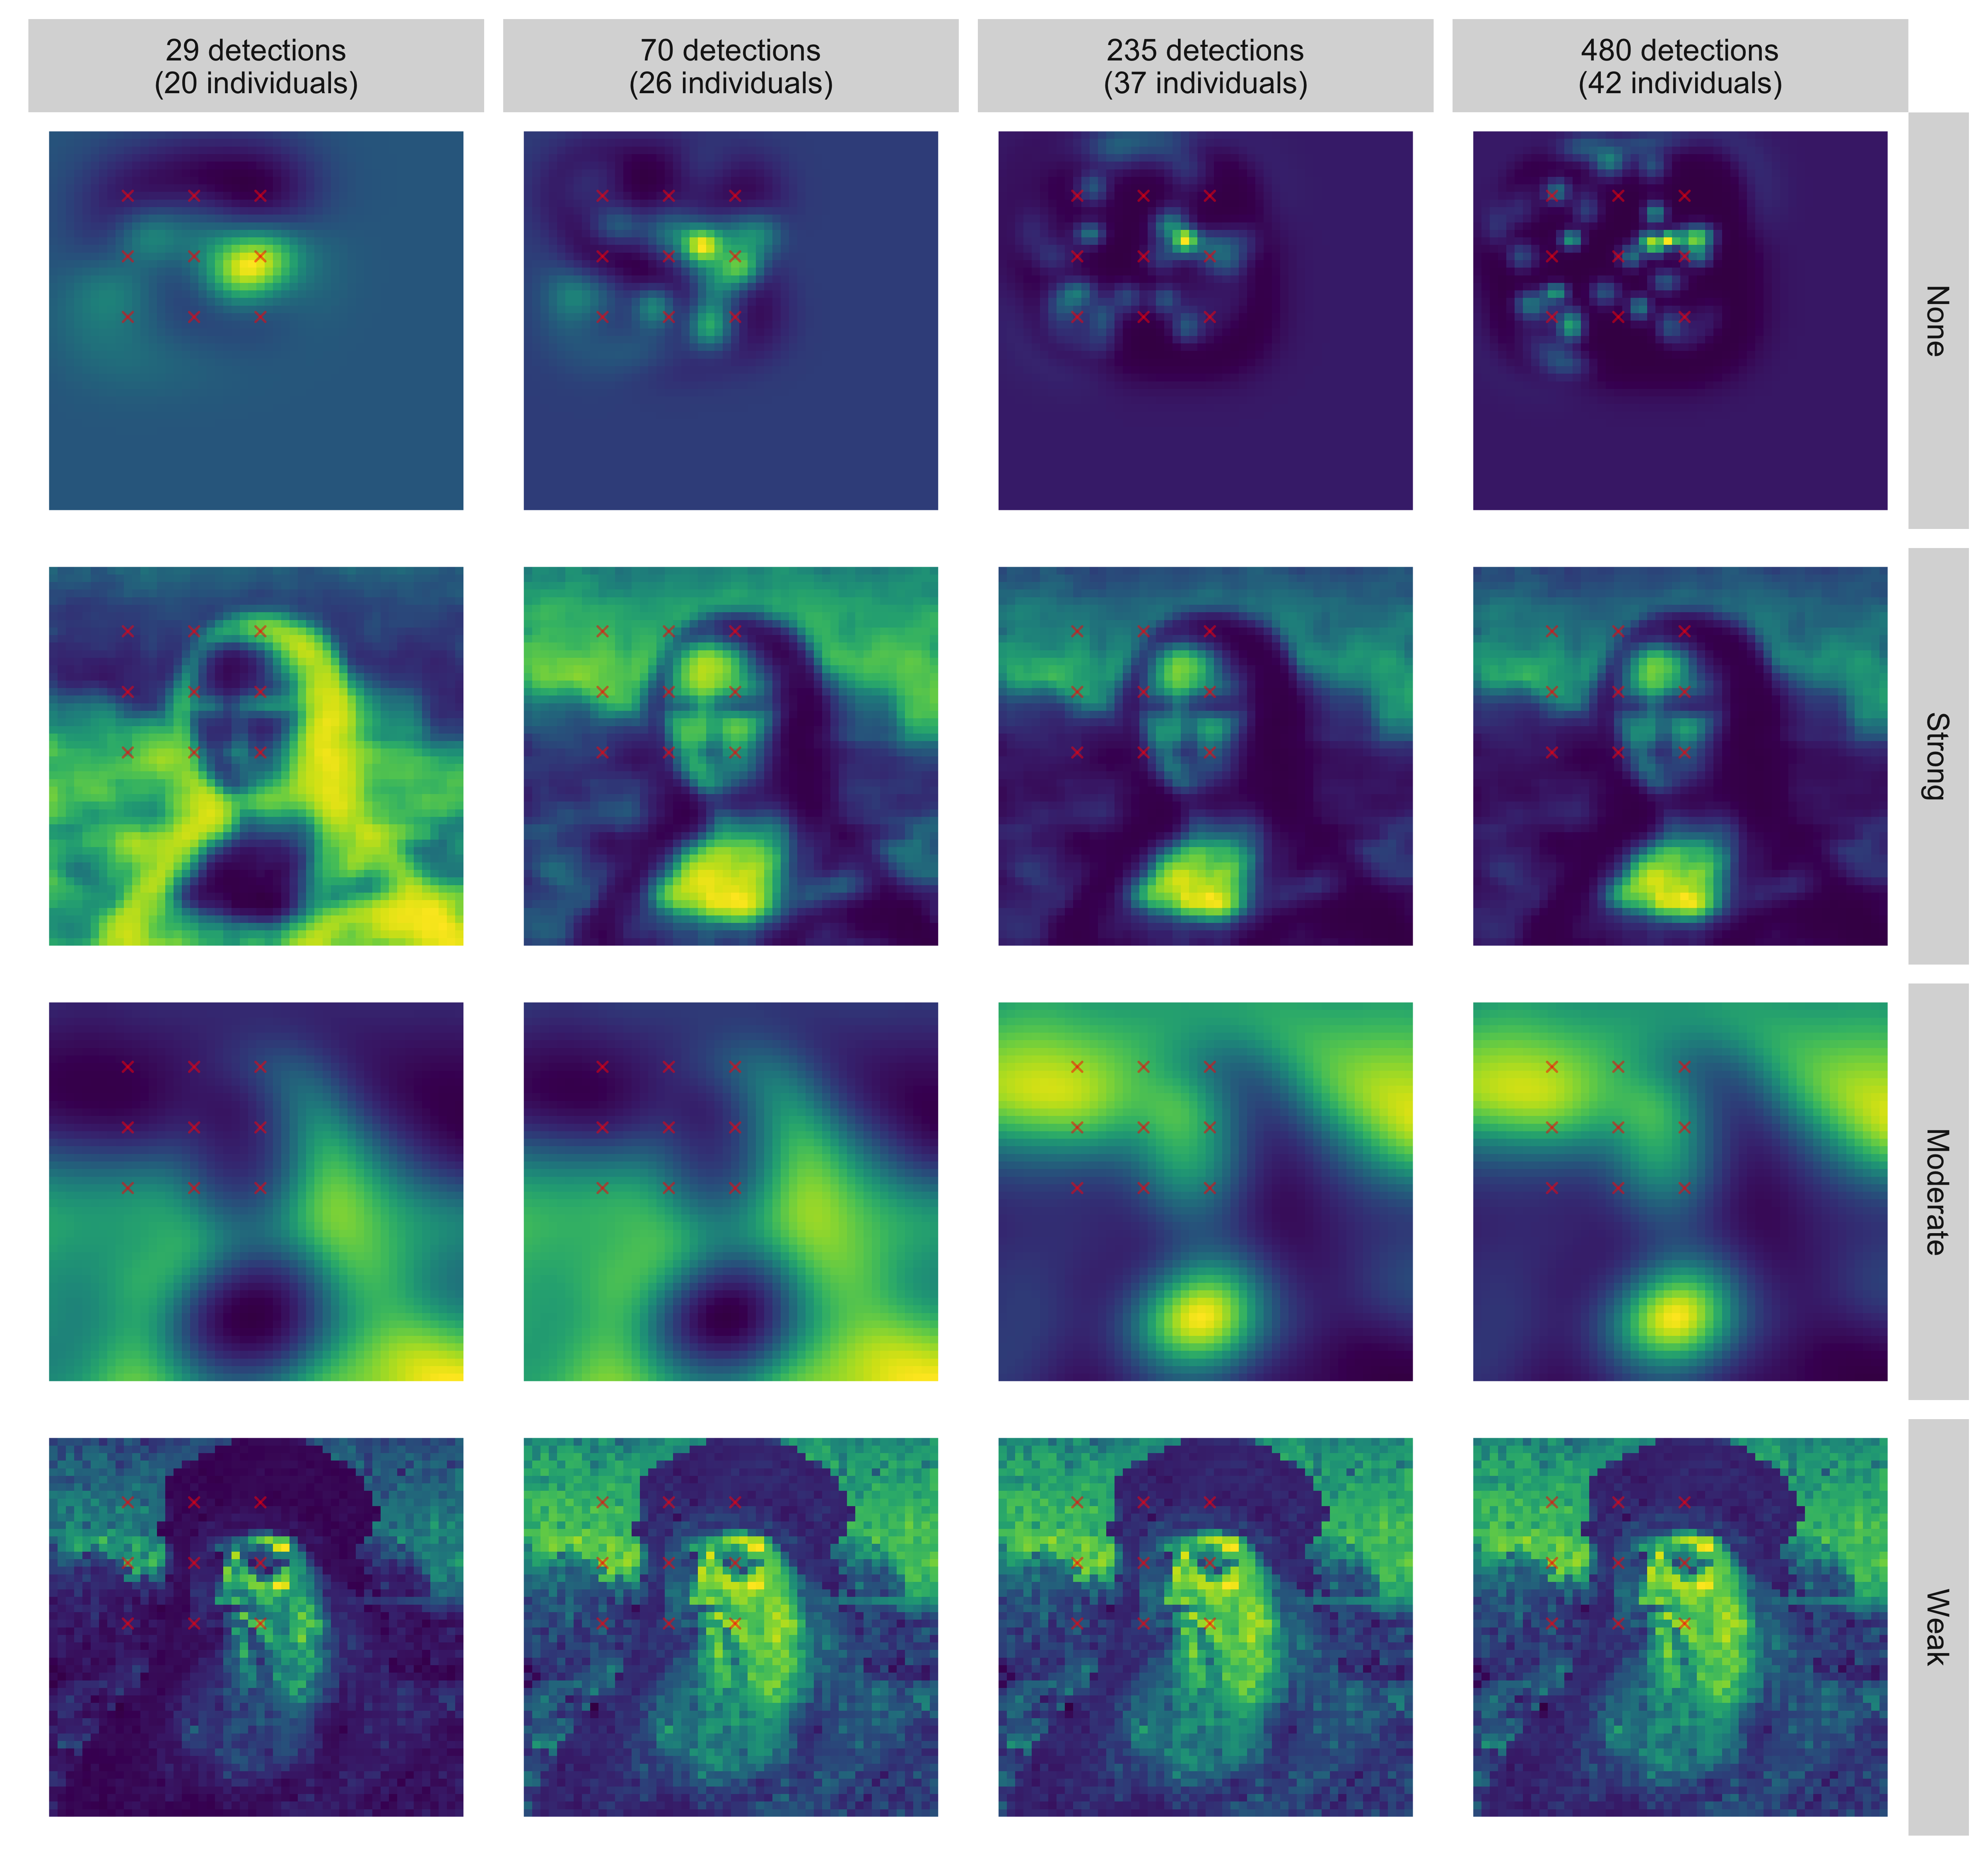
\includegraphics[width=1\textwidth]{mona_peaky.png}
\caption{Estimates of realised activity center density surfaces from a constant density model (first row) and expected activity center density surfaces from a model with density depending on ``strong'' or ``moderate'' covariates (second and third rows respectively, see Section \ref{s:simcapthist} for details of how covariates were simulated). 85 activity centers were generated across the entire image, drawn from a Poisson process with intensity given by the ``Low Res'' image in Figure \ref{mona_inputs}. High density areas are indicated in yellow, low density areas in blue. Detectors are shown as red crosses.}
\label{peaky}
\end{figure}

\subsubsection{Estimated realised animal densities when there are few activity centers}

Estimated realised animal density surfaces -- those that incorporate animal movement -- were smoother than the density surface of estimated realised activity centers and also less sensitive to survey effort (Figure \ref{move}). The estimated realised animal density surface adds a movement kernel that is insensitive to survey effort to a realised activity center surface that becomes more peaked as survey effort increases, so this is to be expected. Estimated realised animal density surfaces were not ``just'' smoothed versions of the realised activity center surfaces, however. In our example unobserved animals were estimated to be spending their time on the outskirts of the study region, far away from any detectors (Figure \ref{move}, second row), which is quite different from the homogenous surface we obtained away from detectors when looking only at activity centers (Figure \ref{move}, first row). In contrast, the realised animal density surface for captured animals {\it was} essentially a smoothed version of the realised activity center surface around the detector array, and so very similar in terms of the broad patterns it showed (Figure \ref{move}, third row).

\begin{figure}[htbp]
\centering
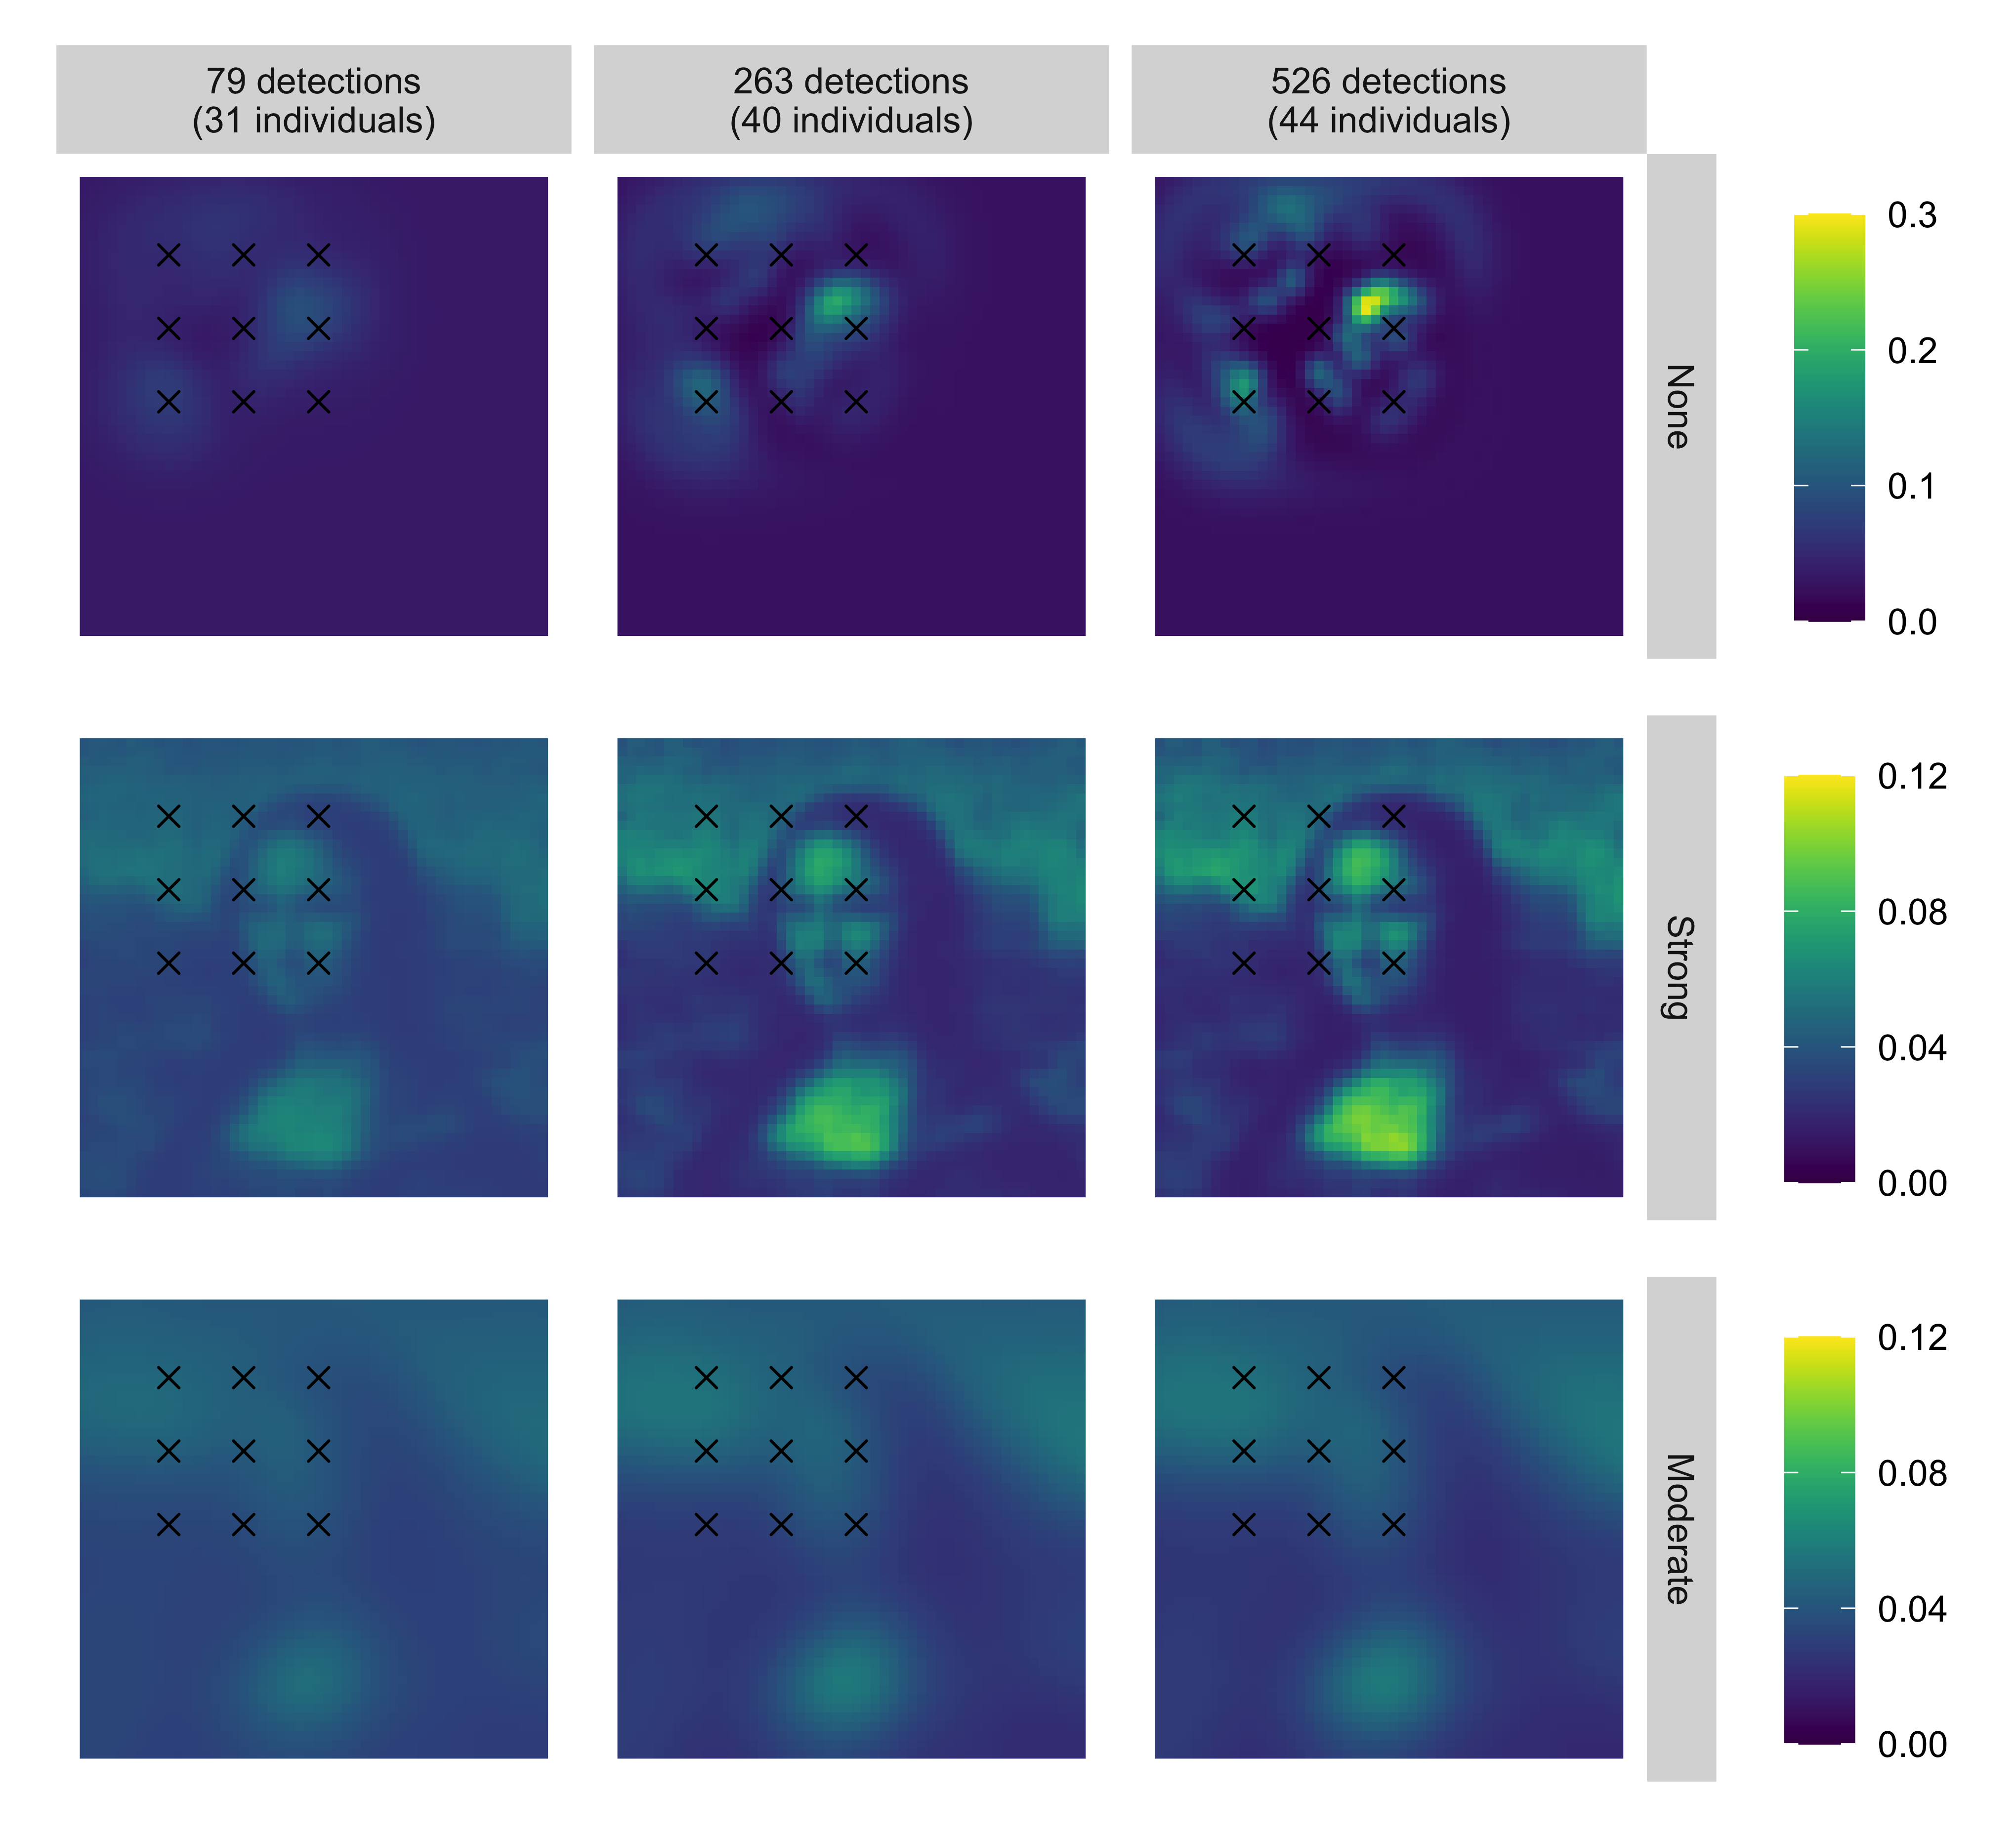
\includegraphics[width=1\textwidth]{mona_with_movement.png}
\caption{Estimates of realised activity center density surfaces from a constant density model (first row) and realised animal density surfaces incorporating animal movement for both observed and unobserved animals (second row) and for observed animals only (third row). High density areas are indicated in yellow, low density areas in blue. Detectors are shown as red crosses.}
\label{move}
\end{figure}


\section{Camera-trap survey of tigers in Nagarahole, India}

\subsection{Materials and methods}
We reanalysed data obtained from a camera trap survey of tigers {\it Panthera tigris} living in and around the Nagarahole Tiger Reserve of Karnataka, India, as reported in \cite{Dorazio+Royle:03}. A full description of the survey can be found in the original reference. The original survey used a spatial array of 162 motion-activated camera traps, these being placed at 2–3 km intervals throughout the area (Figure \ref{tigernocov}, ``All traps''). 

We reanalyzed this data in a likelihood-based framework, first with a model assuming constant density and with three different trap arrays. The first array was the same one employed in the original study. The second was a subset of traps that excluded a large number\todo{say how many and what proportion} traps in the interior of the study region, thus leaving a substantial part of the study area unsurveyed (Figure \ref{tigernocov}, ``Subset \#1''). The third used another subset of traps that excluded eight detectors from each of two interior areas of the survey area in which the original survey showed the density of activity centers to be particularly high (Figure \ref{tigernocov}, ``Subset \#2''). 

We then fitted a number of covariate models in which density was assumed to depend on longitude and latitude. We fitted a variety of linear and smooth functions for each of longitude and latitude; the model selected by the AIC was one including a linear effect of latitude only, and we report results from this model only. Finally, we generated realised animal densities for a constant density model with all traps.

\subsection{Results} 
The same broad patterns were visible in our reanalysis of the Nagarahole tiger survey (Figures \ref{tigernocov} to \ref{tigerspaceuse}). 

\subsubsection{Estimated realised activity center densities}

The full array of traps used in the original Nagarahole study clearly showed three areas of high activity center density in the interior of the study region, along $E\approx 625$ and $N=1324, 1330, 1336$ respectively (Figure \ref{tigernocov}, ``All traps, no cov.''). 

When we reran the survey on a subset of traps that excludes traps in the interior of the study region, high density areas in the interior of the region were replaced by a flat surface indicating a homogenous low density, and the three high density regions described above were not detected  (Figure \ref{tigernocov}, ``Subset \#1, no cov.''). We also observed some regions where estimated density {\it increased} after the removal of the interior traps (see the easternmost detectors in Figure \ref{tigernocov}, ``Subset \#1, no cov.''). This occurs when animals have their activity centers near to, but outside, the area circumscribed by an array -- estimated activity centers then tend to be pulled towards the traps that they are closest to. 

With the second subset of traps, which exclude eight detectors from each of two high density interior areas, the constant density model still recognized that activity centers are located in these areas, but the estimated locations of these activity centers showed a clear shift from what was found in the original survey (Figure \ref{tigernocov}, ``Subset \#2, no cov.''). The estimated location of the northernmost of the two activity centers moved to the south east, while the other activity center moved to the south.

\begin{figure}[htbp]
\centering
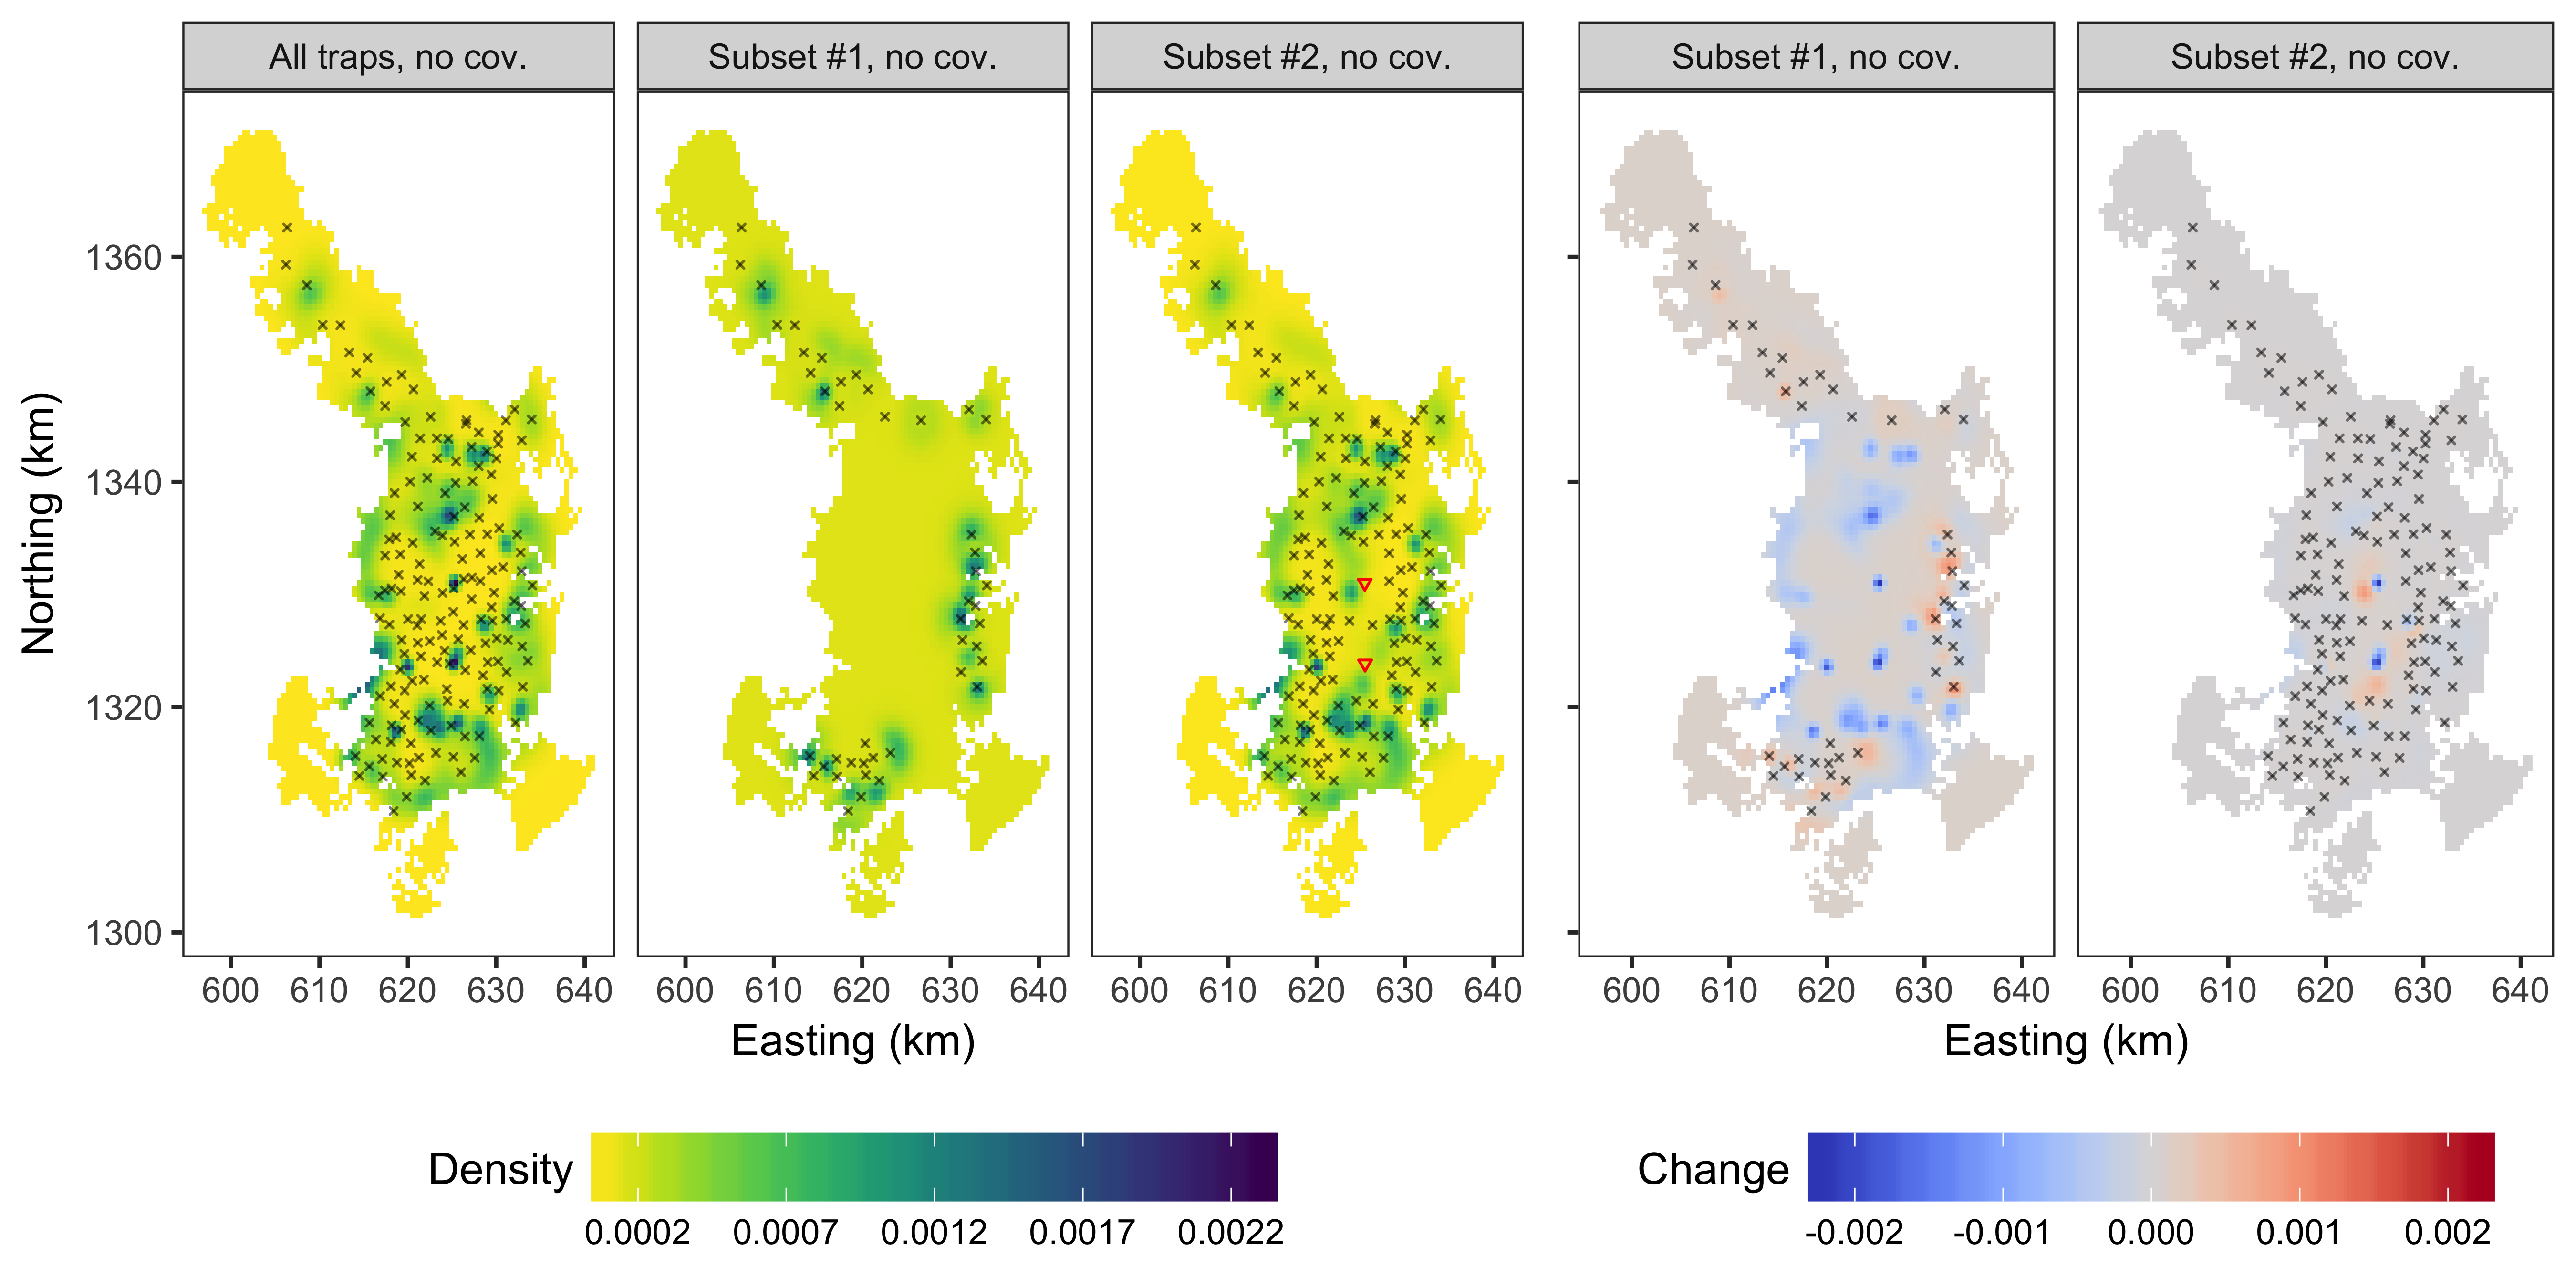
\includegraphics[width=1\textwidth]{tiger_surfaces_nocovs.png}
\caption{Estimated realised activity center densities of tigers in Nagarahole Tiger Sanctuary, India, obtained using different camera trap arrays. Plots (a), (b), and (c) show estimated densities; plots (d) and (e) show differences between the estimated densities obtained using using trap subset \#1 and \#2 and those obtained using all traps. Detectors are shown as black crosses.}
\label{tigernocov}
\end{figure}

\subsubsection{Estimated expected activity center densities}

The model with the lowest AIC was one expressing mean intensity as a linear function of latitude. The estimated density surface obtained from this model showed the estimated mean intensity increasing southwards across the region, with mean intensity in the extreme south roughly four times that in the extreme north (Figure \ref{tigercov}, ``All traps, northing''). Estimates of expected activity center density were much less variable than estimates of realised activity center density, and were also less sensitive to changes in the array of traps, provided that the array provided sufficient coverage of the covariate space to estimate the covariate relationship (Figure \ref{tigercov}, ``Subset \#1, northing'' and `Subset \#2, northing''). 

\begin{figure}[htbp]
\centering
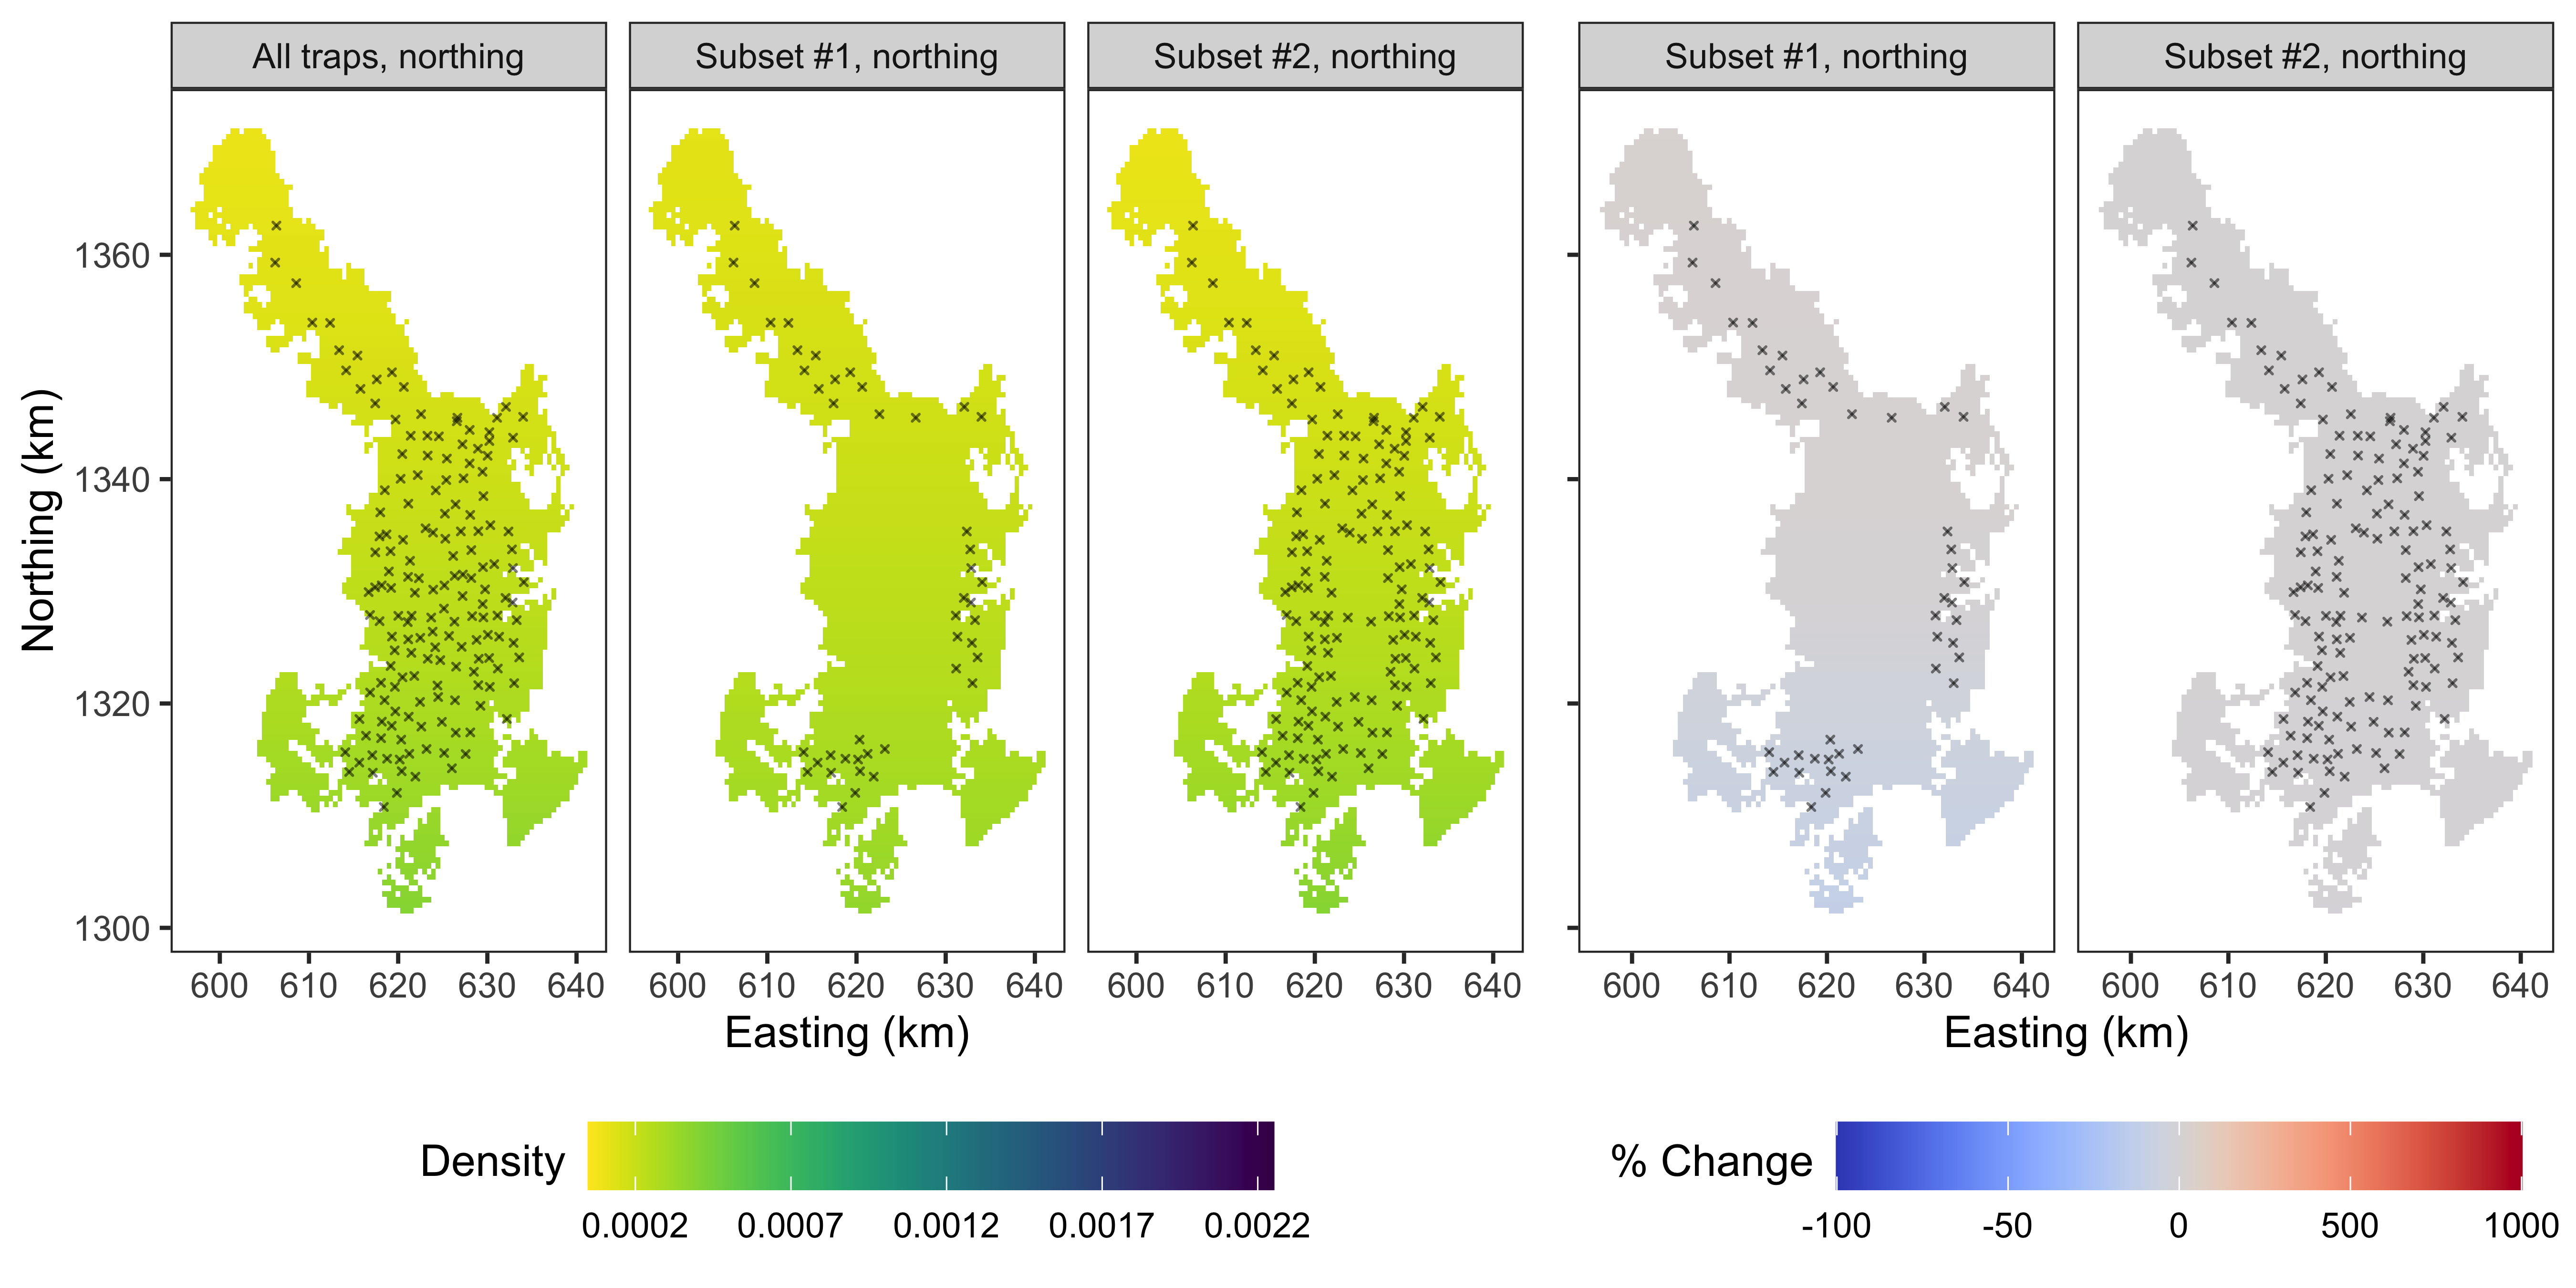
\includegraphics[width=1\textwidth]{tiger_surfaces_covs.png}
\caption{Estimated expected activity center density of tigers in Nagarahole Tiger Sanctuary, India, obtained using different camera trap arrays. Plots (a), (b), and (c) show estimated intensities (expected activity center densities); plots (d) and (e) show differences between the estimated intensities obtained using using trap subset \#1 and \#2 and those obtained using all traps. Detectors are shown as black crosses.}
\label{tigercov}
\end{figure}

\subsubsection{Estimated realised animal densities}

The estimated realised animal density surface differed markedly from the realised activity center density surface, with these differences neatly illustrating the different purposes of the two surfaces (Figure \ref{tigerspaceuse}). Activity center densities were highest in those cells where sufficient information had been gathered to precisely identify where a single tiger's activity center was. Adding movement to the surface had the effect of dispersing each area of high (activity center) density across a much wider area, the extent of which depended on the estimated range of movement. The estimated spatial scale parameter for the fitted half-normal detection function we used was $\sigma=1.85$km, so that animals can move a substantial distance from their activity centers, relative to the size of the study area. As a result, animal density was highest in areas in which there were several activity centers in relatively close proximity to one another, even if the location of these activity centers was less precisely known than other activity centers. This occured in areas near the southern and south-western borders of the reserve, as well as in a central location near $N=1340$ (Figure \ref{tigerspaceuse}). In contrast, animal density was low in areas that contained only a single activity center, even if the location of the activity center was precisely known (for example at $N=1330$, $E=624$).

\begin{figure}[htbp]
\centering
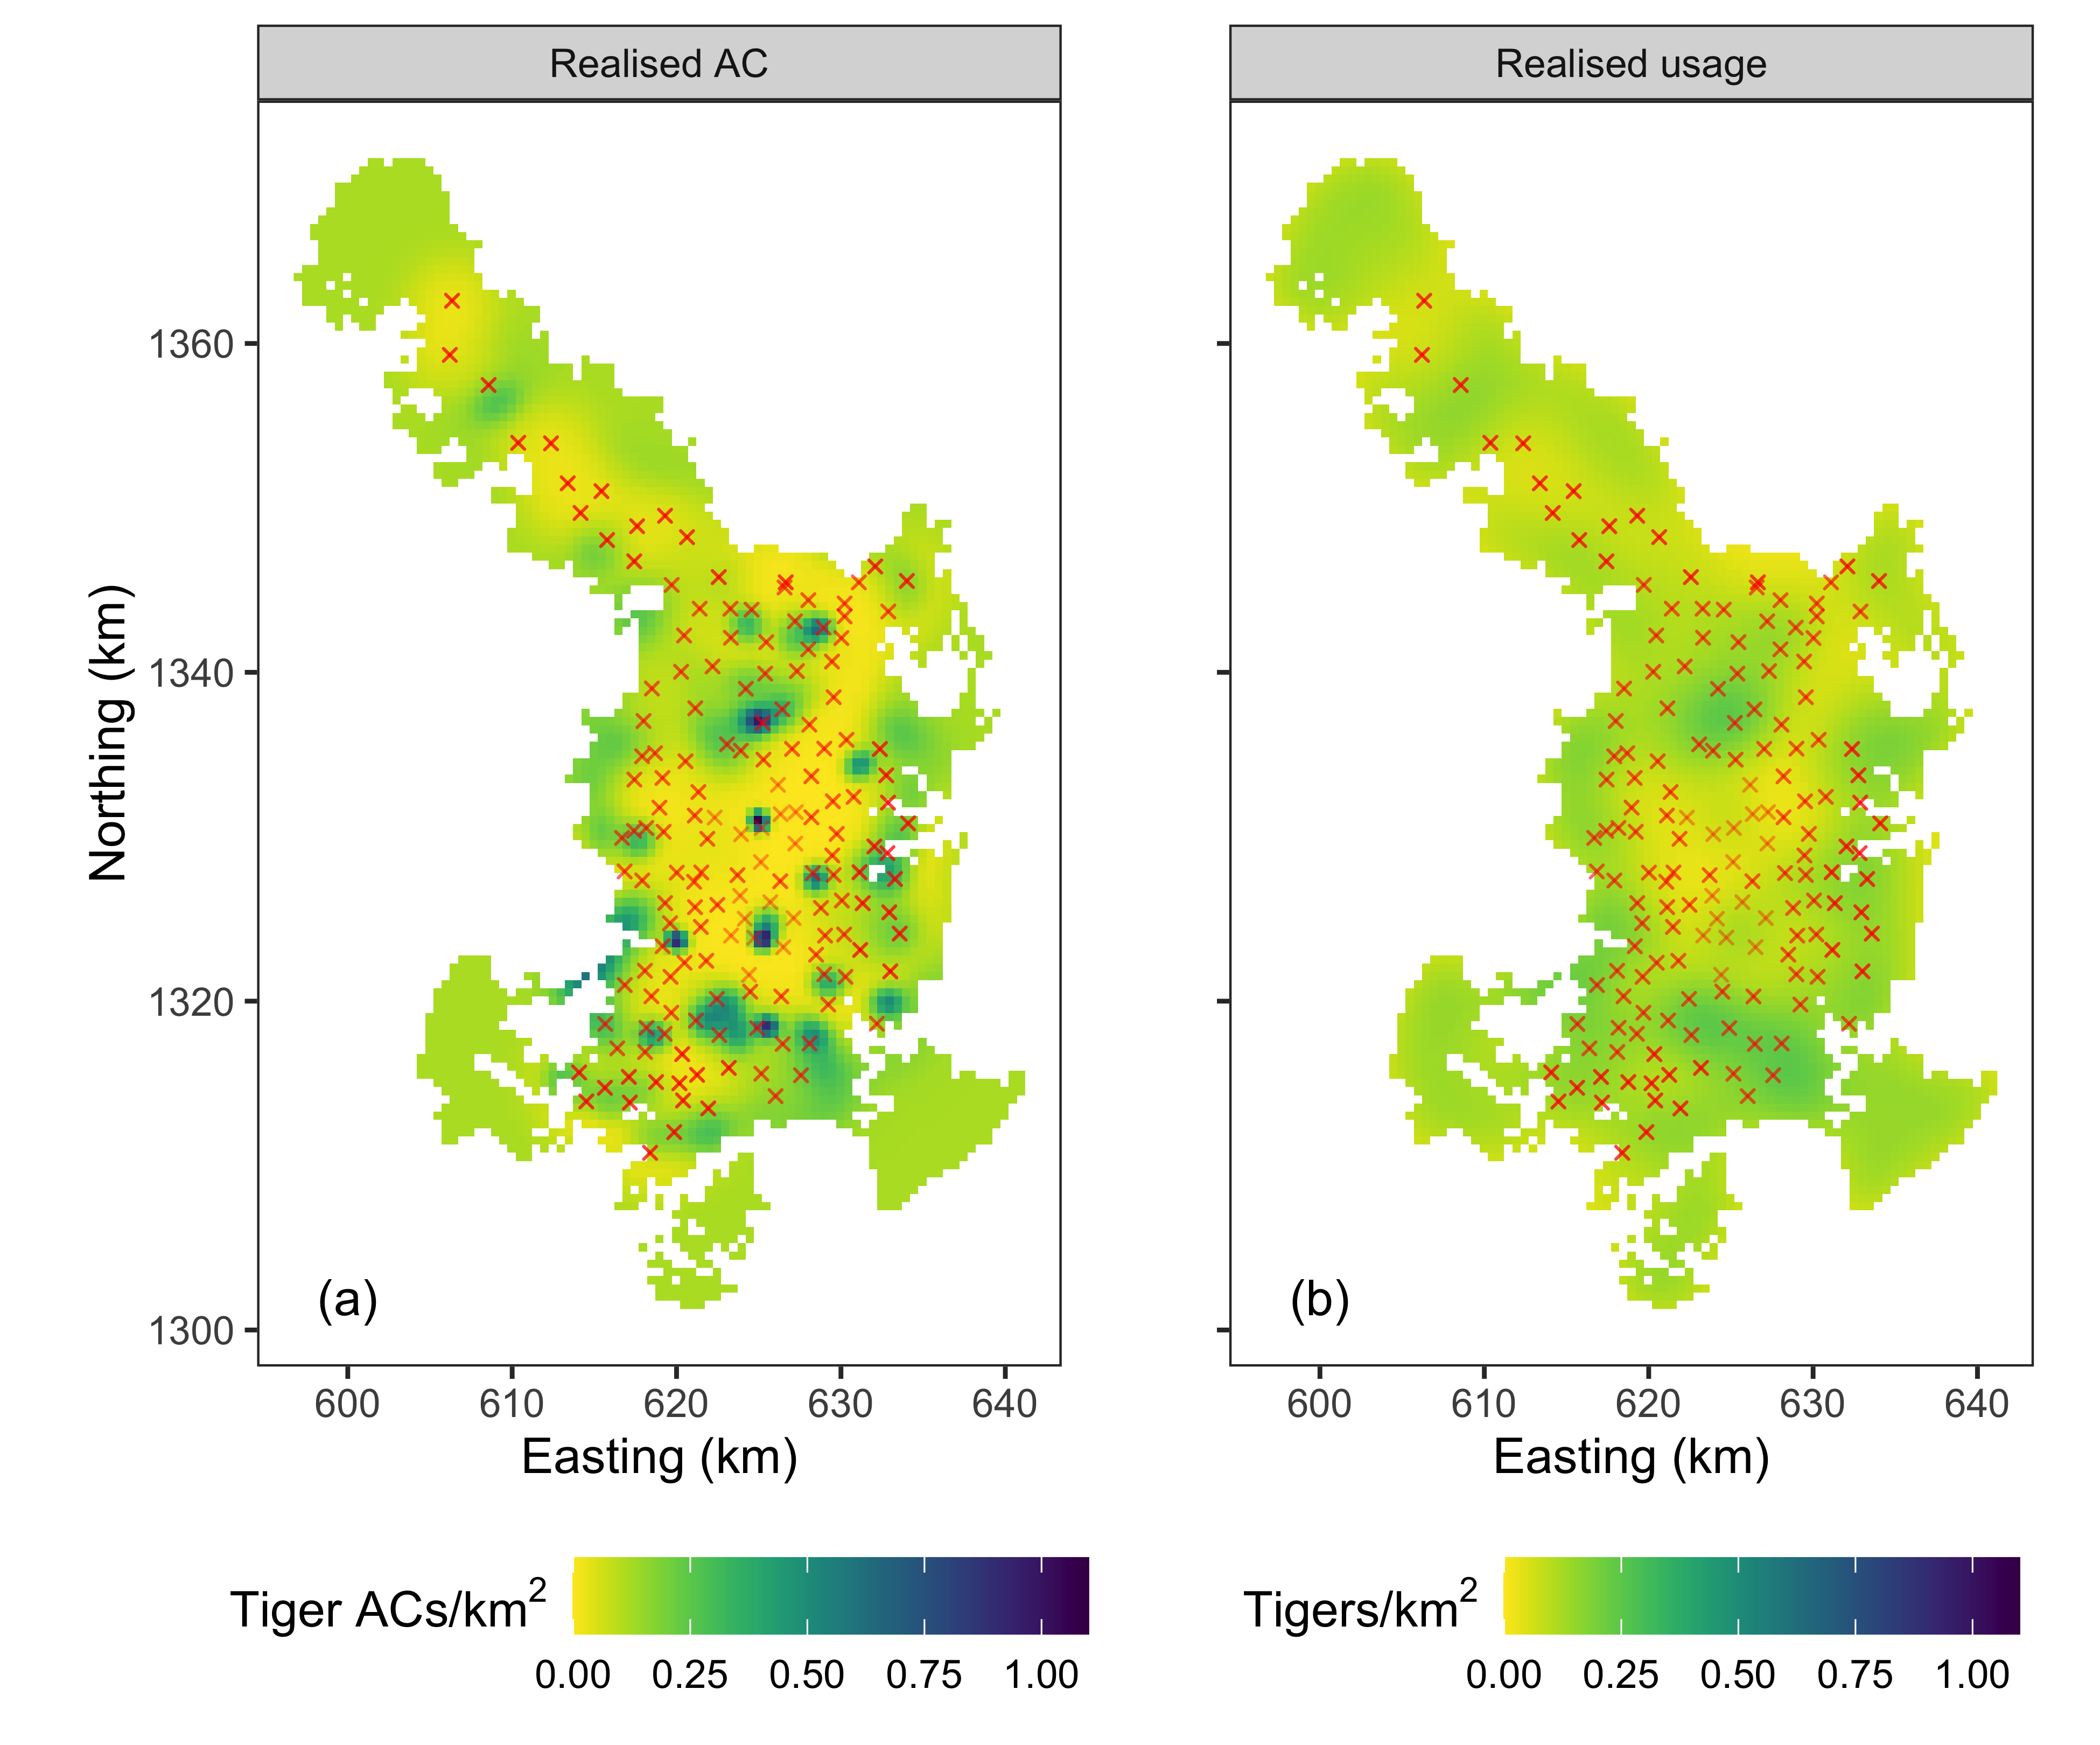
\includegraphics[width=0.6\textwidth]{tiger_spaceuse.png}
\caption{Estimated (a) realised activity center density surfaces from a constant density model and (b) realised animal density surfaces for tigers in Nagarahole Tiger Sanctuary, India. High density areas are indicated in blue, low density areas in yellow. Detectors are shown as red crosses.}
\label{tigerspaceuse}
\end{figure}


\section{Discussion} \label{discussion}
The realised activity centre density obtained from an SCR model cannot be interpreted as a species distribution model. Species distribution models predict where species are likely to occur by correlating environmental covariates with species occurrence or species density. Their rationale is to find favourable habitats and predict that animals will be found in similar habitats across the study region. A species distribution model will tend to place higher densities at locations where environmental covariates are most favourable, and spatial variation in the density surface will depend mostly on how environmental covariates change across space.

In contrast, the density on a realised activity center surface is often placed in spikes where the model is most certain that an activity center is located. The shape and location of these spikes depends on where traps are located and also on survey effort. Different arrays produce quite different results for the same populations\todo[inline]{DLB: I removed these words ``and these results can be improbable, in the sense that high density spikes can occur at locations in unfavourable habitats, if there happen to be activity centers at these locations at the time of the survey.'' as this seems a weak argument to me.} A useful metaphor here is of SCR as a torch shining a light onto the true activity center density surface -- what you see depends on where you shine the torch (trap locations) and how brightly you shine it (survey effort). If you interpret the darkness outside of the beam to mean that everything outside the beam is the same, you fundamentally misunderstand the nature of torches and will draw fundamentally incorrect conclusions.\todo[inline]{DLB: Extended the metaphor with this last sentence, which I think works well?}

Realised activity center surfaces tend to be flat away from where traps are located. It is important to understand that this flatness reflects a lack of knowledge about the density surface away from traps, and does not mean that the density surface is flat away from traps. This point is clearly stated in standard SCR texts\footnote{``As we move away from `where the data live' (away from the trap array) we see that the density approaches the mean density. This is a property of the estimator as long as the detection function decreases sufficiently rapidly as a function of distance. Relatedly, it is also a property of statistical smoothers such as splines, kernel smoothers, and regression smoothers---predictions tend toward the global mean as the influence of data diminishes'' \citep[p165-166][]{Royle+al:13a}} but is misinterpreted whenever researchers explicitly or implicitly treat realised activity center densities as maps of the spatial distribution of activity centers across the study area (unless the study area is very densely surveyed), as is done in \cite{Alexander+al:15}\todo{DLB: Add other examples?}. Another way to see that flatness away from traps reflects uncertainty rather than homogenous density is to plot lower and upper percentiles at each pixel, rather than just the posterior mean -- the differences between these percentiles would be large away from traps and small close to traps. It seems that this is rarely done, or at least reported in the literature; a practice that would be worth changing. 

More importantly for people actually conducting SCR surveys is that the realised density estimates obtained close to traps (and even inside the trap array) {\it also} depend on where traps are located. The inset plots of Figure \ref{mona1low} and \ref{mona1hi} show the same region in space, and this region lies within a $2.5\sigma$ range of all trap arrays, where one would expect to be making inferences about activity centers. We obtained very different density surfaces in this area depending on where traps were located. If one was using SCR to identify areas of high density e.g.\ for conservation purposes, or to locate animals, different areas would be identified depending on which array was used. 

When considering realised activity centres, SCR models answer the question ``where is an animal with {\it this} spatial capture history likely to have its activity center?'' The answer is always contingent on where traps are located. Changing the locations of detectors also changes the expected capture history, and thus the answer to the question of where the activity center is located. This occurs regardless of whether one works in a Bayesian or frequentist framework. Precisely the same is true of the estimated realised activity center density surface, which simply sums estimated activity centers across animals. In this case the question being addressed is ``where are the animals with {\it these spatial capture histories} likely to have {\it their} activity centers?'' The dependency on trap location applies to activity centers estimated for detected animals and for those that were not detected. In the latter case we have limited information and our estimates thus become just ``nowhere near where traps are located''. 

None of this precludes realised activity center surfaces from being useful sources of information, but they do need to be interpreted with care. For practical purposes this means always interpreting them with the caveat that they depend on where traps are located. Realised activity centre densities do not give proper answers to questions like ``where are the high- and low-density regions?'' because the highest and lowest points of the surface will always be at or near traps; not because these are high- or low-density regions of space, but because this is where the capture histories make us most certain that animals are, or are not, present. They also cannot answer questions like ``are animals clustered in space?'' or ``is animal density heterogeneous?'' because the realised density surface will always exhibit variability, even if animal densities are truly a realisation of a homogeneous Poisson point process.

When estimating the location of a given activity center, the bias caused by trap locations is lowest if the activity center occurs near the center of a dense array of traps, and is highest if traps are all on one side of the activity center or if detections are only made at a single trap. Thus bias can be reduced by using a design that makes it likely that all activity centers in the study region are surrounded by a network of traps. This will be unachievable for most wildlife surveys, as it requires a large number of traps covering an area beyond the study region, and ideally placed at random {\it [[[note: I say `beyond the region' so that activity centers at the borders are also in the center of some array, but not sure this is correct -- ????]]]} . In summary, it is incorrect to interpret the realised activity center density surface as if it indicated where animals currently have their activity centers. \todo[inline]{DLB: The paragraph above seems both redundant (we have already made the point about misinterpretation of activity density surfaces quite well I think), and unclear in that I don't know what ``bias'' is being referred to in it. I suggest we remove the paragraph.}

There is a way of using SCR so that it can be interpreted as a species distribution model -- by modelling the mean intensity of the underlying process as a function of enviromental covariates. Covariates allow one to see beyond the spatial extent of the array (see Figure \ref{covariates}), provided that the relationship between covariate and response is a good one, and that traps cover a sufficient range of covariate values to estimate that relationship. The resulting surfaces are no longer strongly tied to one particular realisation of the Poisson process. Rather, they show the (estimated) mean intensity of the underlying process assumed to generate activity centers; in other words, the estimated expected density of activity centers across all realisations. Expected densities will be highest where environmental covariates are most favourable (such as further south in Figure \ref{tigercov}). They  answer the questions ``Where are the high- and low-density regions?'' and ``What spatial variables are good predictors of the high- and low-density regions?'' in a way that is consistent with how this question is answered by species distribution models. They predict where we would expect to see activity centers, if we were able to observe multiple independent populations distribute themselves across the study region. 

Using covariate models, and associated model-based inference, is not without issues -- there is a danger of extrapolating the density surface beyond the range of covariates around the traps, and the relationship with density and covariate is assumed to be the same everywhere as it is around the traps. The extent to which the expected activity center surface predicts where animals have their activity center {\it in this realization} depends on the strength of the covariate relationship and on the number of activity centers, each of which is an independent draw from the underlying process. In the Nagarahole survey, for example, there is a relatively weak northing covariate and a relatively small number of activity centers, and the estimated expected activity center density surface provides very little information about the location of current activity centers. 

The concept of an activity center is central to SCR models, but for many applications of SCR it may be more appropriate to consider a distribution of space use, taking into account all locations where an animal may have been present, rather than a distribution over activity center locations only. The detection function or encounter function estimated as part of an SCR model provides information about how far from its activity center an animal may move. This can be easily integrated with the estimated realised activity center density to give an estimated realised {\it animal} density surface. The resulting surface effectively smooths the realised activity center density surface, with the amount of smoothing determined by the distances that animals move, as given by the detection function. As it is based on activity center locations, the animal density surface also depends on where traps are located and on survey effort. However, it depends less heavily on these factors than the activity center surface because the detection function does not depend on them. In particular, the realised animal density surface quickly stops becoming increasingly ``peaked'' as more survey occasions are added.

Ultimately, the appropriate density surface to use depends on the aims of the researcher. We have argued that the estimated realised activity center density surface should not be used as a species distribution model, because of the strong dependence on trap location and survey effort. But if the goal is to identify the activity centers of {\it some} animals currently in the study region (and it does not matter which ones) then it may well be an efficient way of locating these, particularly at the center of the array. If the goal is to actually {\it find} an animal in the study region, then it is less important where animals have their activity centers and more important to know where they spend their time, and the realised animal density surface \todo{BCS: Should this say ``realised {\bf usage} density instead?} is most useful. If the goal is to estimate where animals (not just the ones in the current realisation) are likely to have activity centers, then this is a species distribution question and the expected activity center surface, with intensity a function of covariates, should be used.

\section{Conclusions}
This paper demonstrates that the summed posterior distribution of estimated ranges across animals obtained from SCR -- what we call the realised activity center density surface -- cannot be used as a species distribution model. We illustrated this point in a number of ways, first with a binomial point process, then by using the Mona Lisa to simulate a Poisson point process, and finally using data from a real-world camera trap survey. All these examples returned the consistent message that realised activity center density surfaces differ depending on trap location. This dependency is most obvious at large spatial scales, where moving a trap array is like ``shining a torch'' on a particular part of the study area, but is also present within the region in and around the trap array itself. Our main messages are:
\begin{enumerate}
\item Realised activity center density surfaces cannot be interpreted as SDMs. This is both because the surface makes inferences about one realisation of a spatial point process, whereas SDMs make inferences about the long run average of the process; and because the surface depends systematically on where traps are located.
\item The realised activity center density surface typically shows highest peaks and deepest troughs close to the center of arrays, defaulting to close to the mean of the underlying process away from the array. A flat density away from traps reflects a lack of knowledge, and not constant density. We should expect some areas away from traps  to show substantial deviations from the process mean -- it is just that we do not know which areas.
\item An SCR model that models mean activity center density as a function of environmental covariates can be interpreted as a SDM. Here the key difference is that the surface obtained from the covariate model -- what we call an expected activity center surface -- is a statement about the mean intensity of the underlying process, and is independent of array location provided that the environmental covariate space has been sufficiently sampled.
\item Realised activity center densities can be extended into realised animal densities by the addition of animal movement. This is done by distributing the probability mass associated with each possible location of a particular activity center across the entire region in which, conditional of that location being the true one, an animal might be detected. The extent of this region is given by the estimated detection function parameters. 
\end{enumerate}

%"OK everyone, put your traps where you'd like to shine your torch, and you'll get a perfectly good estimate of animal density there using our posterior AC map".

\bibliographystyle{mee}
\bibliography{monalisa}

\end{document}
